% T15 of the Transport Papers series.
% 2026-10-08 (interactive session, Claude Opus 5.5, per Leon: "provide a link to
%   the transport papers in the disclaimer ... for all v2.0 papers"). The
%   Authorship and disclosure paragraph now ends with one sentence giving the
%   Transport Papers community on Zenodo, as G01 gives it: "The papers of the
%   series are deposited in the Transport Papers community on Zenodo, \url{...}."
%   No other change; printed version stays 2.0. Recompiled: 22pp (unchanged), 0 errors,
%   0 overfull (unchanged), no undefined references. Script not re-run (no
%   computational content touched).
% v2.0 (2026-10-07, derivation session, Claude Opus 5.5, per rule 20, at Leon's
%   request: knock-ons of T12 v2.0, its Pati-Salam route and the weak angle).
%   Printed version 1.0 -> 2.0 (\date), per Leon. No result added or renumbered,
%   no label changed. rem:valuation: the Standard-Model paper's second branch
%   (M_U 3.4e16, M_I 1.9e10, T12 Prop 10.10), called its "other" or "Pati-Salam"
%   branch to keep "second branch" for rem:branch's; the consistency consequence
%   now on "the two branches on which the couplings meet"; on that branch the angle
%   fixes v_R 4.2e10 and m_D = 1.44 sqrt(f_J) GeV (T12 Prop 11.2), the bottom-
%   like end (top-like needs f_J ~ 4000); the paper keeps both ends (its
%   valuation rests on (U)); M_I lies between the two alpha values, so whether
%   (R) keeps the descent below M_I depends on the end. rem:branch: on that
%   route M_R = v_R f with f shared with the charged fermions (T12 Fact 11.1,
%   Prop 11.5); the texture is not free there and whether this branch is among
%   T12's fits is not settled. prop:leptogenesis(3): "on the conditional
%   branch" -> "on either of the Standard-Model paper's branches". Successor
%   problem (2), Levels (imported), Position and sec:verification follow.
%   Script: verify_T15.py v2.0, three checks added to Part B (B5: the
%   requirement's coefficient from m_3 and v_R, the top-like coupling, the
%   scale ordering), on imported T12 values entered as brackets.
%   Run: verify_T15.py 53/53 PASS (was 50/50), cloud workspace.
%   Compile: pdflatex x3, 22 pages (21 before), 0 errors, 0 undefined refs, 0
%   multiply defined, 0 overfull. Em dashes: 0.
%   Cross-references (rule 21): verify_crossrefs.py T15 34/34 both directions;
%   suite sweep 740 locators, 738 ok; the two failures are pre-existing and outside
%   this pass (T14a line 670, \cite[Premise P2]{ButlerT14}).
% Work-order closure (2026-09-13, per Leon, WORK ORDER T13-KNOCKONS item 1,
%   residual). The order's main charge against fact:democracy, that it
%   imported the alignment with neither of its two conditions, was discharged
%   at v1.1: the indifference instrument is now carried as a structural
%   premise and the Gram-square reading is named. What was still missing is
%   the three-twistor bound: the Fact leans on "the maximal composite" with
%   no bound, no level and no locator, where T13's own fact:bracket states it
%   at observation level with provenance.
%   fact:democracy, first sentence: the faces clause now adds "and the
%     maximality it invokes is the Standard-Model paper's three-twistor
%     bound, imported there and here at the observation level that remark
%     declares".
%   fact:democracy, Provenance: "\cite[Rem.~3.3]{ButlerT12} for the
%     three-twistor bound, at observation level" appended. ButlerT12 is
%     already a bibitem here (fact:content), so no bibliography change.
%   No mathematics, label or number changed; numbering stays frozen per rule
%   21, printed version stays 1.0 per rule 25.
%   Compile: pdflatex x2, 21 pages (unchanged), 0 errors, 0 undefined refs,
%   so T17's status row and verify_T17.py's pages dict need no change.
%   verify_T15.py 50/50. verify_crossrefs.py suite sweep 604/604. Cloud
%   workspace.
% Correction (2026-09-10, mechanical pass, per Leon): rule 23 misidentified T5 as the printed-version exception. T1 is the exception at Version 3.0; every other paper, T5 included, reads Version 1.0. \date corrected accordingly (was 1.1).
% v1.1 (2026-09-10, derivation session, Fable 5.1 subagent, per rule 20,
%   series-review repair pass against series_review_2026-09-09.md).
%   Printed version 1.0 -> 1.1. No mathematics changed.
%   Rule 17, sec:position "Papers that rely on this one": "should read as
%     this version states them" and the instructions to T14 and T17 removed;
%     the paragraph states timelessly what T14 takes (refutation at the
%     scope of prop:seesaw(1), flag covariance with nu_R at grade zero per
%     prop:empty, reheating at Premise (R)) and what T17 takes (that
%     refutation, the seesaw premised under (M), grade zero, rem:branch,
%     Premises (M), (H), (R)); "is now under" -> "holds under".
%   rem:valuation: m_t widened to PDG 2024's 172.57 +/- 0.29, printed as
%     (172.28, 172.86) GeV. The 2e16 ratio recomputed at (33.13, 34.03),
%     printed "33 to 34" unchanged; the 7e14 factor recomputed at
%     (1.1596, 1.1910), printed "1.16 to 1.19 to two places (script-
%     bracketed at (1.159, 1.192))"; M_3 (5.88e14, 6.04e14) and alpha
%     (8.9e12, 9.15e12) unchanged at the printed "6e14" and "9e12".
%   prop:rankone(3): sin^2 th13 bracket -> NuFIT 6.0's (0.0216, 0.0227);
%     m_bb brackets (3.5, 3.9) and (1.3, 1.7) meV unchanged at printed
%     precision (script re-run).
%   Abstract: 248 -> 246 words by whitespace count ("with J the all-ones
%     matrix" parenthesised, "current cosmology" -> "cosmology"); no
%     claim changed. Bibitems checked against the title list: all match.
%   Script: verify_T15.py 50/50. m_t literal (172.28, 172.86); s13sq and
%     the U_tau3 bracket at (0.0216, 0.0227); obs:mixing label drops the
%     unchecked "(42 to 51 degrees)"; the 2e16 ratio check at (33.1, 34.1)
%     and the 7e14 factor check at (1.159, 1.192) plus a check that the
%     endpoints round to 1.16 and 1.19 (both checks failed at the old
%     literals with the widened m_t, as the v1.9 header warned).
%   Compile: pdflatex x2, 21 pages, 0 errors, 0 undefined refs, 0 multiply
%     defined, 0 overfull, no float overflow, 0 em dashes.
% v1.9 (2026-09-09, derivation session, Fable 5.1 subagent, per rule 20,
%   review-repair pass against T15_review_v8.md, same session). No
%   mathematics changed. Compile: pdflatex x2, 21pp, 0 errors, 0 undefined,
%   0 multiply-defined, 0 overfull, no float overflow, 0 em dashes.
%   Script: verify_T15.py, 50/50 exact checks, unchanged (one label: check
%   43 "sits in" -> "lies in"). Numbering frozen: aux diff empty.
%   S1: sec:position "Papers that rely on this one": the prose pass's
%     "supplies this paper with" (for "routes this paper") reversed the
%     T11 and T13 dependencies; now "refers ... to this paper", matching
%     T11 Position (line 806 there) and T13's Koide paragraph.
%   S2: introduction: "parts already derived in the series" (for "on the
%     table") promoted the inputs, which include (S), (U), Conj 3.1 and
%     Premises (M), (H), (R), to derived; now "already present in the
%     series".
%   N1: "the point is essential to the proof" -> "carries the paper's claim
%     that the zero is computed, not forced". N2: rem:currency "confirmed
%     or refuted together" -> "survive or are refuted together". N3:
%     "failure mode". N4: fact:wminusone's condition clause untangled.
%     N5: T17's tables named as T17 names them (refutation table, table
%     of falsifiable claims). N6: script label. N7 (two near-literal
%     pre-existing checks) not rebuilt.
%   KNOCK-ONS for T17 (residual after its 2026-09-08 repair): status row
%     T15 says "rank one under the hierarchy premise (H)"; T15 has rank
%     one at leading order (prop:rankone(0)), (H) governing the sum and
%     the double-beta values, and the row omits the branch alpha << M_3;
%     stance 4's refutation column is one-sided (below the floor only);
%     T15 states the upper limb too (a sum near 0.075 eV, or m_1 above
%     about 4 meV, refutes the number). K1, K6, K8, K10 verified done.
% v1.8 (2026-09-08, prose pass, Fable 5.1 subagent, per project rule 22:
%   mannered prose replaced by literal statement, Leon's ruling to replace
%   the recurring vocabulary too). Compile: pdflatex x2, 0 errors,
%   0 undefined refs, 0 overfull, 0 em dashes; 21pp. Script: verify_T15.py,
%   50/50 exact checks, unchanged (two check labels reworded: "ledger" ->
%   "prediction table", "kill threshold" -> "refutation threshold").
%   Numbering unchanged (aux diff empty). Body only; about 85 sentences.
%   Glossary applied: bet/joint bet/double bet -> prediction (about 30);
%   bet ledger -> prediction table (7); ledger of levels -> levels of the
%   results; tensor ledger / its ledger -> state space (2); T17's ledger ->
%   claim table; kills/kill/killing -> refutes/refutation (12); dies ->
%   is refuted; stakes/staked/staking -> predicts/predicted (5); price ->
%   cost (2); owes/owing nothing to -> uses nothing from (2); owe -> have
%   to record; owns -> in the series; debts declared -> prior work
%   acknowledged; load-bearing -> essential to the proof; machinery ->
%   results; bookkeeping -> computation; frontier -> open problem (2);
%   gated by -> depends on (2); touchpoint -> point of contact; on the
%   table -> derived in the series; honest -> dropped; sits at/lands at ->
%   is at (5); lives in -> lies in; cannot see -> is insensitive to;
%   flavour-blind -> flavour-independent (3); named escape -> the one way
%   the stance could avoid refutation. Non-glossary: silenced -> suppressed
%   (7, incl. prop:leptogenesis title); engine -> mechanism (3); plank ->
%   real-breaking assumption (9); relief valve -> standard way of relaxing
%   the bound (3); squeeze -> bound; casualty -> first to be excluded (2);
%   alive/dead -> allowed/excluded (4); Boltzmann-dead -> -suppressed;
%   dividend -> consistency consequence (3); routes -> supplies (2);
%   content silence -> gap in the derived content; a hair -> slightly.
% v1.7 (2026-09-06, derivation pass after T15_review_v7.md, no blocking
%   findings; Fable 5): Compile: pdflatex x2, 0 errors, 0 undefined refs,
%   0 overfull, 0 em dashes; 21pp. Script: verify_T15.py, 50/50 exact
%   checks, imports GA.py. No mathematics changed.
%   B1: rem:valuation's alpha at the bottom of (U) quoted 5.1e9, matching
%     rem:branch and inside the computed (5.118, 5.477)e9 (was 5e9, below
%     it: the digit review v5's B7 fixed in rem:branch and the v1.6 B3
%     repair re-introduced at this second site).
%   B2: the 7e14 factor check tightened from (1.1, 1.2) to (1.16, 1.19),
%     so "script-bracketed" in rem:valuation and sec:verification points
%     at the bracket the text quotes; message reworded to match. The
%     headroom is deliberately thin (computed 1.16043 to 1.18930, so 0.04
%     and 0.06 percent inside the asserted ends): a refresh of m_t, m_3 or
%     Lambda that moves the factor will fail this check first, which is
%     the intended signal to requote the two figures in the text.
%   KNOCK-ONS: as v1.6's list (K1-K8, K10, N1, N3-N5, N7-N11).
% v1.6 (2026-09-06, derivation pass after T15_review_v6.md, no blocking
%   findings; Fable 5): Compile: pdflatex x2, 0 errors, 0 undefined refs,
%   0 overfull, 0 em dashes; 21pp. Script: verify_T15.py, 50/50
%   exact checks, imports GA.py.
%   B1: the 7e14 factor quoted at its bracket, 1.16 to 1.19, in all three
%     carriers. B2: the non-monotonicity of the exact ratio in M_3/alpha
%     scripted (the value at 176 exceeds those at 66 and 500, so a second
%     root exists between 176 and 500) and listed in Part B. B3: the alpha
%     at which the lowest pairwise crossing sits is given its end (top of
%     (U); three orders above at the bottom). B4: the unification-scale
%     import carries its locator and T12's assembly level in sec:position
%     and in the ledger of levels. B5: lem:breaking's aside restored to one
%     parenthesis; A is general in the main clause.
%   Header correction for v1.5: the calibration tie is a separate check
%     beside the record masses, not a change to check 28.
%   KNOCK-ONS: as v1.5's list (K1-K8, K10, N1, N3-N5, N7-N11).
% v1.5 (2026-09-06, derivation pass after T15_review_v5.md; Fable 5):
%   Compile: pdflatex x2, 0 errors, 0 undefined refs, 0 overfull, 0 em
%   dashes; 21pp. Script: verify_T15.py, 49/49 exact checks,
%   imports GA.py.
%   A1: lem:breaking's "||Pi A Pi|| = 1" clause deleted; the reference
%     direction e_3 e_3^T carries the scale (||Pi A Pi|| = 2/3, lambda_A =
%     4/9), delta quoted relative to it, delta^2 lambda_A rescaling-
%     invariant. B2: the stray w in the proof renamed q.
%   A2: rem:valuation's M_U clause corrected against T12 Prop 6.2: 7e14
%     GeV is the unification-condition scale with the Standard-Model
%     coefficients; the pairwise meetings fall at about 1e13, 2e14 and
%     1e17 GeV; the lowest sits at this paper's alpha, so the leptogenesis
%     dividend is claimed on the conditional branch only (already so in
%     prop:leptogenesis(3)). B11: the sentence given its subject and verb.
%     B3: the unification scale added to sec:position's T12 entry. B4: the
%     factor 1.2 at 7e14 scripted and listed in Part B; "the two values
%     the text names".
%   B1: "nearly two orders (log10 66 = 1.8)" in rem:branch and Premise (R),
%     and in check 43's message (was "one and a half", review v4's slip,
%     carried in good faith). B5: the verification sentence says m_mu/m_tau
%     is used at three figures, and check 28 now ties its target to the
%     script's own lepton masses. B6: "more than a half". B7: alpha at the
%     bottom of (U) quoted 5.1e9. B8: the introduction carries the silence
%     limb. B9: "is met at", with the non-monotonicity and second root
%     named. B10: check 30 in Part B's inventory.
%   KNOCK-ONS: as v1.4's list, plus N11: T12's Position should list T15
%     among the papers relying on its unification section (Prop 6.2).
% v1.4 (2026-09-06, derivation pass after T15_review_v4.md; Fable 5):
%   Compile: pdflatex x2, 0 errors, 0 undefined refs, 0 overfull, 0 em
%   dashes; 20pp. Script: verify_T15.py, 47/47 exact checks, imports
%   GA.py.
%   A1: prop:seesaw(2)'s closing clause, the sixth carrier of the withdrawn
%     bracket claim (missed by review v3's list of five), now reads "which
%     is silent on that bilinear". B7: the three sentences hardening T12's
%     caveat softened to what T12 declares (defined on twistors, undefined
%     for an excited composite, silent on slot-free states). B8: fact:
%     bracket's (1,0) constituents carried with Hypothesis (S), the slot
%     arithmetic noted as unconditional.
%   A2/A3 (the calibration): delta now has a normalisation (relative to
%     the reference direction e_3 e_3^T, ||Pi A Pi|| stated) and is
%     calibrated against the paper's own texture: m_l = c(J + delta_c
%     e_3 e_3^T) reproduces m_mu/m_tau = 0.0595 at delta_c = 0.286 by exact
%     singular values (0.06 gives 0.013). With the neutrino Dirac breaking
%     taken of that size in that direction (an assumption made for the
%     instance, declared), the measured m_2/m_3 needs M_3/alpha ~ 66 by
%     exact diagonalisation: alpha/M_3 ~ 1.5e-2, alpha ~ 9e12 GeV at the
%     top of (U) and 5e9 at the bottom, ONE AND A HALF orders below M_3
%     (was three). rem:branch's recorded relation now stated at leading
%     order with the exact reduction (delta' = 1/66 against 0.024 from the
%     formula, scripted). Premise (R), obs:mixing (tilts about 13 and 3
%     degrees, unscripted) and sec:position (T14 displacement about two to
%     five orders) follow. Supersedes v1.3's 1284, 8e-4, 4.7e11, 2.7e8,
%     "three orders" and "three to six".
%   B1: lem:breaking's remainder written (1 + O(delta) + O(delta^2 M_3/
%     alpha)), the second being O(m_2/m_3) and not vanishing at fixed
%     physical ratio. B6: the domination reason corrected (leading order
%     in delta at fixed alpha, M_3). B2: Premise (H)'s analogy brought into
%     line with the lemma's squaring (a shared direction gives m_1/m_2 ~
%     (m_e/m_mu)^2). B3: Y_Q != 0 in the introduction. B4: 0.1007 meV,
%     pinned in the script. B5: "about 47 degrees at the centre of the
%     bracket", the conversion listed among the unscripted. B9: M_U cited
%     to T12 Prop 6.2 as its conditional branch, with the unconditional
%     7e14 and its factor 1.2 stated; the leptogenesis dividend hedged
%     accordingly. B10: the Gram-square extension in the unchecked list.
%     B11: "about two to five orders" (scripted). B12: citations at each
%     observational input. B13: Fukugita-Yanagida, Davidson-Nardi-Nir and
%     Pilaftsis-Underwood added and the prior art declares the debt. B14:
%     CPT-evenness in the ledger of levels. B15: the bracket sentence
%     names top and bottom masses against the light charged fermions.
%     B16: "33 to 34". B17: checks 5 and 9 listed in Part A. B18: check 43
%     against the closed form cos^2(A e_2, A e_3) for a second A; dead
%     variable removed. B19: the lemma's vector renamed q; the anomaly
%     sums renamed A_3, A_2, A_g, A_c. B20: "four of the six values T12
%     runs"; Yanagida key 1980; HHW pages as T13. B21: stale comments.
%   The v1.3 header's "(H) restated as a condition on the breaking
%     direction" belonged to lem:breaking and rem:branch, not to Premise
%     (H); (H) now carries the squaring itself.
%   KNOCK-ONS FOR OTHER PAPERS (not done here, per rule 20). Outstanding:
%     K1 (subtitle in six bibitems), K2 (T14 "in preparation"), K3/K4 (T14
%     Prop 5.2 wording), K5 (T14 Position short by Prop 5.1 and App. A;
%     Premise (R) at alpha displaces T14 App. A's top-of-range numbers by
%     about two to five orders in T_desc), K6 (T17 refutation row 16), K7
%     (T17 status row: 20pp, 47 checks, Premises (M), (H), (R), the
%     branch), K8 (T17 stance 4), K10 (T17 conditional absence 10), N1
%     (T14's rung-scale valuation uses the seesaw, here under (M)), N3 (T12
%     Position: Props 3.1-3.2), N4 (T11 Position), N5 (T13 Position: Fact
%     2.5, Conj 3.1, Prop 4.4(1), Prop 4.3(4)), N7 (T13's Koide exemption
%     under (M)). NEW: N8 T13 successor (2) has a second dependent (the
%     Gram-square extension to M_R, on which the branch and Premise (R)
%     hang); N9 T13 Prop 4.3(4)/Obs 7.1 and T17's directions row should
%     carry the 42-to-51-degree requirement of obs:mixing; N10 the naming
%     collision ("the empty twistor" is T12's (1,0) doublet and T15's
%     grade-zero singlet; T12's header still says "filled twistor").
% v1.3 (2026-09-06, derivation pass after T15_review_v3.md; Fable 5):
%   Compile: pdflatex x2, 0 errors, 0 undefined refs, 0 overfull, 0 em
%   dashes; 20pp. Script: verify_T15.py, 45/45 exact checks,
%   imports GA.py.
%   A1: review v3 withdraws half of review v2's A1: T12 Prop 3.2's bracket
%     constituents are the slot-occupying (1,0) states at Y = +1/2 each, so
%     its Y = +1 is additive and says nothing about two grade-zero states.
%     fact:bracket's parenthetical deleted and the clause corrected; the
%     five sentences advertising a contradiction (abstract, introduction,
%     rem:different, Premise (M), successor (3)) rewritten to what T12
%     leaves: the bracket is computed only on slot states, undefined
%     beyond them, silent on the neutral bilinear. Premise (M) unchanged
%     in substance. (The v1.2 header's "two empty twistors bracket to
%     e^c's numbers" was the same error and is superseded here.)
%   A2: lem:breaking's eigenvalue consequence corrected: the light masses
%     are (d^2 delta^2/alpha) times the eigenvalues of the COMPRESSION
%     Pi A Pi A^T Pi, not of A Pi A^T (the ranges are not orthogonal; for
%     e_3 e_3^T the two differ by exactly 2/3); the "overlap is O(delta)"
%     clause replaced by the compression argument; the O(delta) correction
%     named as about a quarter at delta = 0.06. rem:branch re-run by exact
%     diagonalisation (the characteristic polynomial factors as lambda
%     times a quadratic, roots by exact square-root brackets): the
%     measured 0.17 at delta = 0.06 needs M_3/alpha ~ 1284, alpha/M_3 ~
%     8e-4, alpha ~ 4.7e11 GeV at the top of (U) and 2.7e8 at the bottom;
%     the instance declared a two-parameter fit, not a test. Header B2 of
%     v1.2 ("alpha is second order") superseded: the .tex's "of the order
%     of the breaking", alpha = delta' M_3, is the statement.
%   A3: prop:empty(2)'s solution set corrected to the two-dimensional span
%     {sY + t(B-L)} with Y_Q != 0, proved by the linear decomposition of
%     the closed form; the ray B-L (Y_N/Y_Q = 3, not in the family) named
%     and scripted; abstract carries Y_Q != 0.
%   A4: the ledger's kill threshold corrected to about 4 meV (certainly
%     4.6 across the bracket), scripted; the bet stated two-sided (B5).
%   A5: the Gram-square extension to the condensate-free M_R flagged as
%     this paper's step in prop:rankone and in the ledger of levels.
%   A6: check 10 rebuilt over an explicit five-state spectrum with N
%     deleted. A7/B8: sec:verification's bracket sentence corrected (the
%     charged-fermion masses and M_U enter at central values) and its three
%     inaccurate check descriptions fixed. B1: obs:mixing states the
%     requirement (|U_tau3|^2 in (0.39, 0.55), 42 to 51 degrees between the
%     heavy eigenvectors) and says the question is open, the order-ten-
%     degree tilt listed as an unscripted estimate. B3: (H) restated as a
%     condition on the breaking direction (m_1/m_2 = lambda'_A/lambda_A).
%     B4: the pair's O(1) injection order carried into (3) and successor
%     (4). B7: "to within about 0.1 meV (0.105 at the boundary)". B9: the
%     elimination check now compares against an independent Gaussian
%     solve. B10: the instance check separated from the measured bracket
%     in sec:verification. B11: check 23 folded (charged-lepton form
%     included), the bald literal removed, check 39's window narrowed.
%     B12: script tag prop:doublebet. B13: v named and valued; lambda_A
%     restated; m_mu/m_tau printed where delta ~ 0.06 is justified; the
%     A S A^T notation removed. B14: inverted floor 0.098; "rank one at
%     leading order" in abstract and introduction; the beta != 0
%     parenthesis; m_3 bracket (49.4, 50.5). B15: M_U bracket dropped from
%     the factor sentence. B16: fact:ceiling notes T14's valuation uses the
%     seesaw, here under (M). B17: "mechanism"; flavour-blindness named as
%     this paper's reading at observation level and listed in the
%     exclusions; the LN extension acknowledged to reach past the
%     excited-composite caveat. B18: the flag-covariance clause says T14
%     states it for the grade-three state and the argument transfers.
%     B19: the displacement of T14's seeding numbers sized in sec:position.
%     B20: T13 Prop 4.3(4) cited beside Obs 7.1; HHW attributed to the
%     quark case. B21: T10's own confrontation carried into fact:wminusone
%     and prop:doublebet. B22: LEGEND quoted as a 10-20 meV band. B23: T11
%     and T13 added as relying papers; T17's rows named.
%   KNOCK-ONS FOR OTHER PAPERS (not done here, per rule 20). Outstanding
%     from v1.2: K1 (the subtitle in six bibitems: T11, T12, the T12 lepton
%     note, T13, T14, T17), K2 (T14 "in preparation"), K3/K4 (T14 Prop 5.2:
%     grade-three, compositeness floor), K5 (T14 Position short by Prop 5.1
%     and App. A; Premise (R) at alpha displaces T14 App. A's top-of-range
%     numbers by two to six orders in T_desc, the floor scaling as
%     T_desc^(3/4)), K6 (T17 refutation row 16), K7 (T17 status row: empty
%     twistor, Y computed, seesaw premised, 20pp, 45 checks,
%     Premises (M), (H), (R) and the branch), K8 (T17 stance 4), K10 (T17
%     conditional absence 10: two values under (H) and the real plank, the
%     hull 1.3-3.9 meV without). Moot: K9, K11, K12. NEW: N1 T14 Prop 6.4
%     and Position: its rung-scale valuation uses the seesaw, here under
%     Premise (M); N3 T12 Position: T15 also imports Props 3.1-3.2; N4 T11
%     Position: T15 imports Thm 5.6(1), (2), (5), Rem 5.10, Prop 4.1 and
%     reads the incidence relation for the dimensions; N5 T13 Position: T15
%     also imports Fact 2.5, Conj 3.1, Prop 4.4(1), Prop 4.3(4); N7 T13's
%     Koide exemption (line ~701) assumes seesaw-composed neutrino masses,
%     now under Premise (M). Series housekeeping: DESI DR2 has three
%     bibitem forms under two keys across T10, T15, T17.
% v1.2 (2026-09-06, derivation pass after T15_review_v2.md; Fable 5):
%   Compile: pdflatex x2, 0 errors, 0 undefined refs, 0 em dashes; page
%   count: 18pp. Script:
%   verify_T15.py rewritten, 41/41 exact checks; imports GA.py;
%   every observational input bracketed.
%   A1 (the charge rule): the rule "a bracket's charge is the sum of its
%     constituents' charges" is NOT T12's and is contradicted by T12 Prop
%     3.2 (two empty twistors bracket to Y = +1). prop:seesaw(2) now proves
%     the elementary gauge-invariance statement outright (a bilinear's
%     hypercharge is the sum of the two fields' hypercharges; N N is the
%     unique neutral fermion bilinear of the derived content; L N carries
%     -1/2) and says in terms that it owes nothing to the framework's
%     bracket. NEW fact:bracket imports T12 Props 3.1-3.2 in T13 Fact 2.1's
%     form (two empty twistors bracket to e^c's numbers; the relation to
%     the order parameter is unsettled). Premise (M) now also carries that
%     the framework realises the field-theory Majorana term at all.
%     Abstract, introduction and rem:different rewritten accordingly.
%   A2 (Premise (H)): restated at the strength the consequences use,
%     m_1/m_2 below about 0.01 (m_1 below about 0.1 meV), which the
%     charged-sector analogy supplies (0.002 to 0.005); (2) and (3) state
%     the m_1 residue with script-certified values at m_1 = 0.1, 1, 3,
%     10 meV; the ledger's kill threshold corrected (m_1 above 1 meV moves
%     the sum off the floor; above 3 meV past the 0.064 eV bound).
%   A3/A4/B5 (alpha): the Gram-square reading gives M_R proportional to J
%     at leading order, so alpha = 0 there and is second order; the paper
%     takes the alpha << M_3 branch explicitly (rem:branch).
%     prop:rankone(0) is proved on the democratic 2x2 block needing only
%     M_3 != 0 (alpha = 0 allowed). NEW lem:breaking (PROVED, scripted):
%     with m_D = d(J + delta A) the light matrix is exactly
%     (d^2 delta^2/alpha) A Pi A^T + (d^2/3M_3) w w^T, so
%     m_2/m_3 = (delta^2 lambda_A/9)(M_3/alpha)(1 + O(delta)); the measured
%     0.17 is reached with delta ~ 0.06 and alpha/M_3 ~ 1.5e-3 (instance
%     certified). Premise (R) restated at alpha, the LOWER heavy scale; the
%     exactly degenerate pair at alpha named as the resonant configuration
%     that alignment does not silence, its O(1) prefactor scripted; the
%     abstract says "silenced under a reheating premise". The like-for-like
%     comparison with the charged ratios withdrawn.
%   A5: the "only CP violation" clause restated at T14's level (the
%     orientation is the only CP-violating datum the framework supplies,
%     uniqueness not claimed there, a relaxing theta-angle unexcluded) and
%     flavour-blindness argued where the step needs it.
%   A6: fact:democracy carries T13 Conj 3.1 (faces = families, conjectural),
%     the indifference instrument as a structural premise (T13 Fact 2.5),
%     and face-valuedness with its locator (T13 Prop 4.4(1)); the S3
%     invariance of M_R tagged at structural level in prop:rankone and in
%     the ledger; the LN extension named as this paper's.
%   A7/A8: checks 8, 9, 12, 13, 29 rebuilt (the singlet deleted from the
%     spectrum; the Z6 condition as a function with an off-lattice
%     failure; the block elimination assembled and the small eigenvalue
%     certified against m_D^2/M with its error; the interference term with
%     a complex breaking phase, zero at 0 and pi and nonzero off them).
%     Every observational input bracketed (angles, m_t, m_b, m_*, M_U,
%     m_3, Lambda); the prose numbers scripted; T14's hedge reinstated
%     with the exclusion list extended.
%   A9: the sixteenth refutation restated scale-free. In T11's conventions
%     [omega omega] is an area times a momentum (fact:join carries the
%     dimensional reading); the Lambda term is below the flat term by
%     Lambda l^2/6 for a composite of extent l, which reaches one only at
%     l = sqrt(2) L_H; for constituents at the neutrino's own scale the
%     Lambda-term neutrino has extent 2^(1/4) L_H exactly. "Thirty-one
%     orders" withdrawn everywhere. B7: the Casimir branch disposed of
%     (C ~ 2e63 needed, scripted).
%   A10: Position section in the sibling form with T-numbers and cites.
%   A11: prop:doublebet recast as an Observation (label kept as
%     prop:doublebet for inbound refs); the editorial sentences moved to
%     rem:currency.
%   B1 abstract trimmed. B2 quoted ratios inside their brackets (K ~ 45,
%     about 33, about 6e4). B3 m_bb values quoted at the computed brackets
%     with the angles bracketed. B4 notation: Y_D for the Yukawa matrix,
%     bold m_D for the matrix and m_D for its eigenvalue, S for the lemma's
%     matrix, (tau, iota) lattice indices, J glossed, m_* in the statement,
%     delta and varphi defined, the sign convention stated once. B6
%     inverted ordering reworded. B8 the T12 name collision noted. B9
%     T12's parenthetical carried. B10 T11 v1.5 (Facts carry no versions,
%     as in the siblings). B11 T11 Thm 5.6(1) cited. B12 T12's own run of
%     the family acknowledged. B13 the splittings printed with brackets
%     and a global-fit locator (NuFIT 6.0). B14 a double-beta limit and a
%     next-generation projection cited. B15 the model of each of the
%     bounds stated. B16 "fifth stance" (the capstone's numbering). B17
%     pointer to rem:valuation; T10 clause (ii) carried. B18 the block
%     elimination written out; the U_e2, U_e3 identifications stated;
%     script t-values consistent. B19 labels ("leading-order scalar
%     seesaw"; the floor is kinematic for any m_1 >= 0; "one nonzero
%     entry in that basis"; the eigenplane choice arbitrary, two bases
%     scripted). B21 tags; the mixing paragraph is obs:mixing; "alignment
%     result". B22 fig:bet referenced; the line drawn at the framework's
%     value with the floor bracket shaded. B24 the anomaly solution set
%     in closed form (prop:empty(2) now proves the family IS the solution
%     set for Y_Q != 0) with Witten's anomaly named. B25 the abstract says
%     the numbers are consequences of m_1 = 0 and real phases.
%   KNOCK-ONS FOR OTHER PAPERS (not done here, per rule 20): K1 the
%     subtitle in the T15 bibitem of T11, T12, the T12 lepton note, T13,
%     T14, T17 (now "The Empty Twistor, the Seesaw Scale, and the Bet at
%     the Floor"; "Derived Seesaw" is a withdrawn level claim); K2 T14's
%     bibitem "in preparation"; K3/K4 T14 Prop 5.2: "the grade-three
%     state" should read the hypercharge-zero singlet, and "the
%     compositeness floor" should read the cosmological term of the
%     deformed bracket (the locator T15 Prop 4.1 still resolves); K5 T14's
%     Position section should list Prop 5.1 and App. A among T15's
%     imports, and Premise (R) is now at alpha, below the ceiling, so T14
%     App. A's "at the ceiling or below it" is read at "below" here; K6
%     T17 refutation row 16 (the Lambda term, not a floor; the seesaw is
%     premised, not derived; no "thirty-one orders"); K7 T17 status row
%     T15 (empty twistor, grade zero; Y computed not forced; Premises (M),
%     (H), (R); page and check counts); K8 T17 stance 4 (attribute 0.052
%     and 0.092 to Hou, Wang, Zhao and Zhang, not DESI; under Premise (H);
%     drop the priority claim); K9 T17 numbers delta_CP as stance 5 and T15
%     now agrees; K10 T17 conditional absence 10 (two values under (H) and
%     the real plank, the hull 1.3-3.9 meV without); K11 T13's Position
%     names Obs 7.1 as an import of T15, now cited here; K12 T12 successor
%     (6): T15 records the (S) dependency in sec:position.
% v1.1 (2026-09-05, derivation pass after T15_review_v1.md; Fable 5):
%   Compile: pdflatex x2, 0 errors, 0 undefined refs, 0 em dashes; 15pp.
%   Script: verify_T15.py rewritten, 29/29 exact checks, imports GA.py.
%   The identification re-founded on T12 v1.5 Prop 5.3(3) and Thm 5.5(2):
%   nu_R is the hypercharge-zero singlet at GRADE ZERO in T12's listing,
%   the EMPTY twistor; subtitle changed; prop:filled -> prop:empty. The
%   withdrawn floor replaced by fact:join (T11 v1.5 Thm 5.6, Rem 5.10).
%   fact:ceiling cites T14 Prop 6.4 with Hypothesis (U) and the range.
%   lem:s3 (PROVED) resolved the rank of M_R. Premise (H); two double-beta
%   values; Facts restated; locators; Position section; bib; the mixing
%   sentence inverted.
% 2026-08-24: renumbered (was T22) and retitled per Leon; content unchanged.
% v1.0 (sprint 2, 2026-08-21): M6: assembly pass; final abstract; one
% rule-13 figure (fig:bet); AWAITING REVIEW. v0.1-v0.4: M1-M5.
% House rules: no em dashes; short abstract; standard series disclaimer;
% physics touchpoints kept (rule 10); proof standard per rule 11 (Fact
% (imported) discipline); verification imports GA.py (rule 12); diagrams
% per rule 13; Position in the series (rules 15, 18); timeless body (rule 17).
\documentclass[11pt]{article}
\usepackage[margin=1.1in]{geometry}
\usepackage{amsmath,amssymb,amsthm,mathtools}
\usepackage{booktabs}
\usepackage[dvipsnames]{xcolor}
\usepackage{tikz}
\usepackage[colorlinks=true,linkcolor=MidnightBlue,citecolor=MidnightBlue,urlcolor=MidnightBlue]{hyperref}

\newtheorem{theorem}{Theorem}[section]
\newtheorem{proposition}[theorem]{Proposition}
\newtheorem{lemma}[theorem]{Lemma}
\newtheorem{corollary}[theorem]{Corollary}
\theoremstyle{definition}
\newtheorem{definition}[theorem]{Definition}
\newtheorem{remark}[theorem]{Remark}
\newtheorem{example}[theorem]{Example}
\newtheorem{conjecture}[theorem]{Conjecture}
\newtheorem{fact}[theorem]{Fact}
\newtheorem{observation}[theorem]{Observation}
\newtheorem{question}[theorem]{Question}
\newtheorem{premise}[theorem]{Premise}

\newcommand{\Cl}{\mathrm{Cl}}
\newcommand{\R}{\mathbb{R}}
\newcommand{\C}{\mathbb{C}}
\newcommand{\T}{\mathbb{T}}
\newcommand{\Mat}{\mathrm{M}}
\newcommand{\End}{\operatorname{End}}
\newcommand{\tr}{\operatorname{tr}}
\newcommand{\id}{\mathrm{id}}
\newcommand{\ip}[2]{\langle #1, #2\rangle}
\newcommand{\br}[1]{\langle #1\rangle}
\newcommand{\mnu}{\Sigma m_{\nu}}
\newcommand{\J}{\mathbf{J}}
\newcommand{\mD}{\mathbf{m}_{D}}
\newcommand{\LH}{L_{H}}

\title{\bfseries Neutrino Masses\\[4pt]
  \large\itshape The Empty Twistor, the Seesaw Scale, and the Bet at the Floor}
\author{Leon Butler\\ \normalsize\href{mailto:lbutler.math@gmail.com}{\texttt{lbutler.math@gmail.com}}\\ \normalsize ORCID: \href{https://orcid.org/0009-0006-4449-5617}{0009-0006-4449-5617}}
\date{Version 2.0, October 2026 \textperiodcentered{} Transport Papers, T15}

\begin{document}
\maketitle

\begin{abstract}
\normalsize
We identify the right-handed neutrino as the hypercharge-zero state of the framework's derived content, the empty twistor at grade zero, and prove that anomaly cancellation could not have fixed its hypercharge: with a fourth singlet free and $Y_{Q} \neq 0$, the anomaly-free spectra are exactly the span of $Y$ and $B - L$. The cosmological term of the deformed bracket cannot supply the neutrino mass (the sixteenth refutation: it lies below the flat term by $\Lambda l^{2}/6$ at extent $l$). Gauge invariance makes the Majorana bilinear of the total singlet the one mass term needing no condensate, a textbook fact about which the framework's own bracket, computed only on slot states, says nothing; with its scale a premise, the seesaw follows. Indifference makes the Majorana matrix $S_{3}$-invariant, hence $\alpha\mathbf{1} + \beta\J$ ($\J$ the all-ones matrix), aligned with the democratic Dirac matrix, and the light matrix is rank one at leading order with $m_{3} = m_{D}^{2}/M_{3}$: normal ordering, and, as consequences of $m_{1} \approx 0$ and real phases, the sum at the oscillation floor $\mnu \approx 0.059$ eV and $m_{\beta\beta}$ at $1.5$ or $3.7$ meV. That sum is at the centre of the sharpest tension in cosmology, and the framework, which predicts $w = -1$, cannot relax the bound in the standard way: one joint prediction. Leptogenesis is suppressed under a reheating premise at the cost of a registered stance, $\delta_{CP} \in \{0, \pi\}$. Tier B/C with every premise named, a prediction table, and exact machine verification.
\end{abstract}

\medskip
\noindent\textbf{MSC 2020.} Primary 81V15, 81V25; Secondary 83F05, 15A18.\\
\textbf{Keywords.} right-handed neutrino; seesaw mechanism; neutrino mass ordering; cosmological neutrino mass bound; neutrinoless double-beta decay; leptogenesis; leptonic CP phase.

\newpage
\textbf{Authorship and disclosure. }The founding idea of the series is the author's: that division by zero in a Clifford algebra should be read not as a prohibition but as a transport into a higher-dimensional algebra, and that the transported division need not be accompanied by an inverse operation. The direction of investigation and the critical review of the results are likewise the author's. The mathematical development and the drafting of the text were carried out in extended collaboration with Claude Fable 5 (Anthropic), an AI system. The papers of the series are deposited in the Transport Papers community on Zenodo, \url{https://zenodo.org/communities/transport-papers}.

\newpage
\section{Introduction}\label{sec:intro}

The neutrino was the largest gap in the framework's derived content. This paper addresses it using only parts already present in the series, and ends by registering the framework's most precise and most exposed prediction: this is, by design and by declaration, the series' fastest-falsifiable paper, published while the prediction is still open.

The chain. The Standard-Model paper T12's derived content always contained a fourth colour singlet: the single-twistor sector carries \emph{two} singlets, at grades zero and three of $\Lambda^{\bullet}\C^{3}$, and the observed comparison column always had two. The right-handed neutrino is the grade-zero state, the \emph{empty twistor}, the pair system with no rung occupied, whose hypercharge the weight rule computes as zero. Anomaly cancellation could not have fixed it: with a fourth singlet of free hypercharge and $Y_{Q} \neq 0$ the anomaly-free spectra are exactly the two-dimensional span of the derived spectrum and $B - L$, a fact we prove in closed form, so the zero is a computation of the content derivation and not a consistency condition, and the Standard Model's ambivalence about $\nu_{R}$ is the ambivalence of a bottom-up construction that has only anomalies to go on. The natural small-mass mechanism is refuted first (the sixteenth refutation): the cosmological term of the mass paper T11's deformed bracket lies below the flat term by $\Lambda l^{2}/6$ for a composite of extent $l$, and can dominate only at horizon size. Gauge invariance then singles out the Majorana bilinear of the total singlet as the one fermion mass term that carries no charge and needs no condensate, an elementary fact proved outright and using nothing from the framework; whether the framework's own mass bracket, which T12 computes only on slot states and about which it says nothing for slot-free states, realises that term, and at what scale $M$, is a premise this paper names rather than derives, and with it the light masses follow by block inversion. Indifference makes the Majorana matrix $S_{3}$-invariant, which we show means $\alpha\mathbf{1} + \beta\J$ with $\J$ the all-ones matrix and, in the Gram-square reading, $\alpha = 0$ at leading order: the democratic vector is an eigenvector, and the seesaw of the democratic Dirac matrix is rank one at leading order and scalar on the democratic block, $m_{3} = m_{D}^{2}/M_{3}$, whatever $\alpha$ is. Three numbers follow: the ordering is normal (inverted excluded by rank plus small corrections, not by fit); the sum is bounded below by the oscillation floor and is at it, $\mnu \approx 0.059$ eV, if the second stage of the breaking is hierarchical; and the effective double-beta mass is one of two values, $1.5$ or $3.7$ meV, if the breaking is real. These are consequences of $m_{1} \approx 0$ and real phases, shared with any model having those two features; what the framework adds is the structure that produces them. The sum is at the exact centre of the sharpest tension in current cosmology, and the framework cannot use the community's standard way of relaxing the bound (a varying dark-energy equation of state) because it predicts $w = -1$: the two stances are one joint prediction. Finally, the heavy states that make the masses are the textbook mechanism of leptogenesis, and that mechanism is suppressed in three steps (alignment, a reheating premise at the lower heavy scale, phases), at the cost of a fifth registered stance: $\delta_{CP} \in \{0, \pi\}$.

\subsection*{Prior art}

The prior work, acknowledged once. The seesaw mechanism is classic \cite{Minkowski1977, GRS1979, Yanagida1980, MohapatraSenjanovic1980}; what the framework adds is the identification of the state that carries it, a proof of which parts of the mechanism are forced by gauge invariance and which are premises, and an $S_{3}$-invariant texture with consequences. That anomaly cancellation with a right-handed neutrino leaves hypercharge undetermined up to $B - L$ is textbook, and T12 already exhibits the family and runs it at four values; we prove in-paper that the family is the whole solution set, because the argument is short and the point carries the paper's claim that the zero is computed, not forced. The oscillation splittings and angles are the global fits' \cite{PDG2024, NuFIT2024}; the cosmological bounds and their tensions \cite{DESI2025, HouWangZhaoZhang2026}, the long-baseline record \cite{T2KNOvA2025}, and the double-beta limits and projections \cite{KamLANDZen2023, LEGEND2021} are the experimental record's, refreshed at submission and tracked in the prediction table of Section \ref{sec:bets}. Democratic mass matrices are the flavour literature's \cite{HHW1978}, inherited through the families paper T13 \cite{ButlerT13}. The leptogenesis results of Section \ref{sec:bets} (the decay-asymmetry interference formula, the washout parameter and equilibrium mass, the resonant enhancement of a degenerate pair, and the asymmetry a successful mechanism needs) is standard and is imported at that level \cite{FukugitaYanagida1986, DavidsonNardiNir2008, PilaftsisUnderwood2004}. What this paper claims as new is the identification of $\nu_{R}$ as the empty twistor, the sixteenth refutation at its exact scope, the $S_{3}$-invariance lemma and the exact rank-one seesaw it yields with the breaking relation that follows, the three numbers with their premises named, the joint prediction with the dark-energy stance, and the three-step suppression of leptogenesis with its falsifiable phase corollary.

\subsection*{Contribution}

(1) The empty twistor: $\nu_{R}$ identified, its hypercharge computed, and the proof that anomalies could not have computed it (Section \ref{sec:empty}). (2) The sixteenth refutation at its scope, the gauge-invariance computation with its premise named, the $S_{3}$ lemma, the exact rank-one seesaw and the breaking relation: ordering, the sum, the double-beta values (Section \ref{sec:seesaw}). (3) The joint prediction with $w = -1$, and leptogenesis suppressed, with the fifth stance (Section \ref{sec:bets}). (4) The prediction table: what decides each stance, and when (Section \ref{sec:bets}). (5) Machine verification of every computational identity in exact arithmetic, with the exceptions listed \cite{ButlerVerifyT15}.

\section{Setting and imports}\label{sec:setting}

\begin{fact}[imported: the derived content and its singlets]\label{fact:content}
The minimal massive hierarchy's fermion content is $(2,3) \oplus (2,1)$, the doublets under the Standard-Model paper's Hypothesis (S); the single-twistor sector $\Lambda^{\bullet}\C^{3} = 1 \oplus 3 \oplus \bar{3} \oplus 1$, graded zero through three, carries the weight $q = -2k$ at grade $k$ and hence the hypercharge $Y = -k/3$, that is $0, -\tfrac13, -\tfrac23, -1$, unconditionally as a computation on the single-twistor Fock space with the pair-slot factor acting alone (that Fock space is not a subspace of the tensor state space, and under (S) it is the row $j = 0$); listed by the handedness that keeps the even grades, the singlet spectrum is $(1)_{0} \oplus (\bar{3})_{-2/3} \oplus (\bar{3})_{+1/3} \oplus (1)_{+1}$, that is $\nu^{c}, u^{c}, d^{c}, e^{c}$, with the hypercharge-zero singlet at grade zero; the four anomaly conditions hold on this spectrum, and determine it (up to the $u^{c}, d^{c}$ relabelling) given the content, $Y_{Q} = \tfrac16$, and a fourth singlet of hypercharge zero or none; and the physical representations are confined to the $\mathbb{Z}_{6}$ lattice. \emph{Provenance:} \cite[Prop.~5.1, Prop.~5.3, Thm.~5.5, Thm.~4.2]{ButlerT12}; Hypothesis (S) is declared there and is open.
\end{fact}

\begin{fact}[imported: the mass bracket and its quantum numbers]\label{fact:bracket}
A massive matter unit is a two-twistor composite whose flat mass is the bracket, $m^{2} = 2|\br{\pi^{1}\pi^{2}}|^{2}$ at $\Lambda = 0$. The bracket transforms by $\det(U)$ under the internal $U(2)$, and under the global form with the hypercharge of Fact \ref{fact:content} the bracket of two twistors, each the vacuum of its pair system, transforms as $(1,1)$ with $Y = +1$: the quantum numbers of $e^{c}$, and not those of a weak doublet. The constituents there are slot-occupying states (that paper's $(1,0)$ components, which exist in its state space under Hypothesis (S), each of hypercharge $+\tfrac12$, so that the $+1$ is their sum; the slot arithmetic $\lambda^{3}$ per slot is unconditional in the global form), not the slot-free grade-zero state this paper calls the empty twistor; the bracket is defined on such twistors, is computed there only for that case, is not defined for an excited composite, and says nothing, either way, about a bilinear of two grade-zero states. The relation between this object and the Standard Model's order parameter is not settled in the series, and the reading of the bracket as an order parameter is recorded at observation level only. \emph{Provenance:} \cite[Props.~3.1-3.2]{ButlerT12}; \cite[Prop.~4.1]{ButlerT11}; the form of this Fact is the families paper's \cite[Fact~2.1]{ButlerT13}.
\end{fact}

\begin{fact}[imported: indifference, the faces, the democratic alignment, and the rank-one texture]\label{fact:democracy}
The indifference instrument forbids uncaused structure (distinctions nothing in the framework determines); it is a structural premise of the series, not a theorem, and is flagged as such wherever it is used. The identification of the three generations with the three two-twistor faces of the maximal composite is the families paper's Conjecture 3.1, at conjectural level, and the maximality it invokes is the Standard-Model paper's three-twistor bound, imported there and here at the observation level that remark declares; the mass bracket is face-valued, one bracket per face, so a vacuum is a direction in the three-dimensional face space, and its alignment is what breaks $S_{3}$ (structural level). Under the instrument the condensate's source lies on the democratic line spanned by $u = (1,1,1)/\sqrt{3}$, and, under the Gram-square reading of the leading mass form, the leading Yukawa form is $Y_{0} \propto \J = u'u'^{\mathsf{T}}$ with $u' = (1,1,1)$ and $\J$ the $3 \times 3$ all-ones matrix, of spectrum $(3, 0, 0)$: one heavy family and two light at leading order, lifted by the second-order breaking $S_{3} \to S_{2} \to 1$ that converts the CKM shape into CKM numbers. \emph{Provenance:} \cite[Fact~2.5, Conj.~3.1, Prop.~4.3, Prop.~4.4(1)]{ButlerT13}, each at the level stated there; \cite[Rem.~3.3]{ButlerT12} for the three-twistor bound, at observation level.
\end{fact}

\begin{fact}[imported: the exact join, and the absence of a floor]\label{fact:join}
For two twistors $Z^{1}, Z^{2}$ and the frozen point $I_{\Lambda}$ with $\lambda = \Lambda/6$, the composite's deformed bracket is $B_{\Lambda} = \br{\pi^{1}\pi^{2}} + \tfrac{\Lambda}{6}[\omega^{1}\omega^{2}]$ and its squared mass is $m^{2} = 2|B_{\Lambda}|^{2} + \tfrac{\Lambda}{3}C$ with $C \ge 0$ the internal Casimir, which vanishes exactly when the Gram matrix is scalar; for $\Lambda > 0$ the massless locus is $B_{\Lambda} = 0$ with scalar Gram matrix, and it is neither empty nor the doubled locus, so compositeness by itself sets no lower bound on mass. In that paper's conventions the incidence relation is $\omega = \mu_{x}\pi$ with $\mu_{x}$ linear in the point, so with $[\br{\pi\pi}] = $ mass one has $[[\omega\omega]] = \text{length}^{2} \times \text{mass}$: an area times a momentum, numerically a length in natural units but not a distance. \emph{Provenance:} \cite[Thm.~5.6(1), (2), (5), Rem.~5.10]{ButlerT11}; the dimensional reading is taken from that paper's incidence relation and mass formula.
\end{fact}

\begin{fact}[imported: the ceiling under Hypothesis (U), the arrow, and the flag covariance]\label{fact:ceiling}
The dark-matter paper's rung scale is its Hypothesis (U): that the rank-one eigenvalues of the different sectors coincide at the ceiling, so that the neutrino's Dirac eigenvalue there equals the common leading-order value; under (U) the seesaw $m_{3} = m_{D}^{2}/M_{R}$, used there as standard physics and available here only under Premise (M) below, values $M_{\mathrm{rung}} = M_{R} = m_{D}^{2}/m_{3}$ from the observed $m_{3}$ in the range $m_{b}^{2}/m_{3} \approx 3.5 \times 10^{11}$ GeV to $m_{t}^{2}/m_{3} \approx 6 \times 10^{14}$ GeV, the ends being the two readings of (U), with the alignment of Fact \ref{fact:democracy} explicitly never equating magnitudes across sectors (this is a fit of the same quantity from the same datum as Remark \ref{rem:valuation} below, and is read there). The descent's asymmetry is inherited initial data, a declared stance, universal over the oriented towers by that paper's Premise P4 (a theorem for the mirror, void for the odd towers); the orientation is the only CP-violating mechanism the framework itself supplies, uniqueness among all conceivable mechanisms not being claimed there, with a relaxing $\theta$-angle named as unexcluded. The identification of $\nu_{R}$ with a singlet grade is flag-covariant (the flag conjugate exchanges the two singlet grades wholesale; that paper states this for the grade-three state, and the argument transfers unchanged to the grade-zero state this paper identifies), so no completion of the orientation can exclude it; this holds under Hypothesis (S) and with the gauge sector's CPT-evenness as a premise there. The descent reheating $T_{\mathrm{desc}}$ is taken there at the ceiling or below it. \emph{Provenance:} \cite[Prop.~6.4, Prop.~5.1, Prop.~5.2, App.~A]{ButlerT14}.
\end{fact}

\begin{fact}[imported: the registered $w = -1$, and its condition]\label{fact:wminusone}
On the Einstein region the frozen point's norm cannot vary, so $w = -1$ there (proved); off it the naive extension of the identification does not give a constant on a matter-dominated cosmology, and a definition of the frozen point that made the norm track $R/12$ would be refuted already; if dark energy is that norm and the frozen point admits a definition on a matter-filled region that keeps it parallel, then $w = -1$ exactly at every epoch, with no parameter to absorb a deviation: a registered stance, conditional on that definition, which that paper names as the one way the stance could avoid refutation, and does not use. That paper records its own confrontation: the second baryon-acoustic data release reports a preference for an evolving equation of state at roughly three to four standard deviations, contested on three grounds and not a detection, and the stance takes no comfort in the dispute. \emph{Provenance:} \cite[Prop.~4.2(i)-(iii) and the confrontation recorded there]{ButlerT10}.
\end{fact}

\section{The empty twistor}\label{sec:empty}

\begin{proposition}[The empty twistor]\label{prop:empty}
Three statements.
\begin{enumerate}
\item \emph{(The identification; imported.)} The single-twistor sector of Fact \ref{fact:content} carries two colour singlets, at grades zero and three, and the observed comparison column ($\bar{3} \oplus \bar{3} \oplus 1 \oplus 1$) always contained two: the right-handed neutrino was in the comparison from the start. In the Standard-Model paper's listing, $\nu_{R}$ (as $\nu^{c}$) is the grade-zero state of the single-twistor sector, the \emph{empty twistor} in this paper's usage (T12 uses the same phrase for the one-slot, no-pair doublet state, a different object), the pair system with no rung occupied, and its hypercharge is $Y = -0/3 = 0$ by the weight rule; the grade-three state, the filled twistor, has $Y = -1$ and is $e^{c}$ after conjugation. Where the Standard Model treats $\nu_{R}$ as optional, this content carries it necessarily.
\item \emph{(Anomalies could not have fixed it; proved.)} For the content $Q = (2,3)$, $L = (2,1)$, $u^{c}, d^{c} = (1,\bar{3})$, $e^{c} = (1,1)$ and a fourth singlet $N$ of hypercharge $Y_{N}$, all in one handedness, with $Y_{Q} \neq 0$, the solutions of the four anomaly conditions ($[SU(3)]^{2}U(1)$, $[SU(2)]^{2}U(1)$, gravitational, cubic) are \emph{exactly} the two-dimensional span $\{sY + t(B - L)\}$ with $Y_{Q} = \tfrac{s}{6} + \tfrac{t}{3} \neq 0$, up to the relabelling $u^{c} \leftrightarrow d^{c}$, where $Y$ is the derived spectrum with $Y_{N} = 0$ and $B - L$ takes the values $\tfrac13, -\tfrac13, -\tfrac13, -1, 1, 1$ on $Q, u^{c}, d^{c}, L, e^{c}, N$; up to normalisation this is the family $Y + t(B - L)$, with $Y_{N} = t$, together with the ray of $B - L$ itself, on which $Y_{N}/Y_{Q} = 3$. So anomaly cancellation leaves $Y_{N}$ free, and the zero of (1) is a computation of the content derivation, not a consistency condition. With $Y_{N} = 0$ imposed the family collapses to the derived spectrum (Fact \ref{fact:content}), which is why the Standard-Model paper's uniqueness theorem carries that hypothesis. (Witten's global $SU(2)$ anomaly imposes nothing here: the doublet count is even and a singlet does not enter it.)
\item \emph{(Anomaly-invisible, on the lattice; proved.)} At $Y_{N} = 0$ the fourth singlet contributes to none of the four sums, so deleting it from the spectrum changes none of them, and the $\mathbb{Z}_{6}$ lattice admits its entry. The orientation dependency of the identification is discharged by the flag covariance of Fact \ref{fact:ceiling}.
\end{enumerate}
\end{proposition}

\begin{proof}
(1) is Fact \ref{fact:content}. (2) Write $(a, b, c, d, e, f)$ for the hypercharges of $(Q, u^{c}, d^{c}, L, e^{c}, N)$ with multiplicities $(6, 3, 3, 2, 1, 1)$. The four sums are $A_{3} = 2a + b + c$, $A_{2} = 3a + d$, $A_{g} = 6a + 3b + 3c + 2d + e + f$, $A_{c} = 6a^{3} + 3b^{3} + 3c^{3} + 2d^{3} + e^{3} + f^{3}$ (the letter $A$ for anomaly sum, local to this proof). The three linear conditions give $d = -3a$, $b + c = -2a$, $e = 6a - f$. Put $p = bc$; then $b^{3} + c^{3} = (b + c)^{3} - 3p(b + c) = -8a^{3} + 6ap$, and the cubic condition becomes $6a^{3} + 3(-8a^{3} + 6ap) - 54a^{3} + (6a - f)^{3} + f^{3} = 18a\,(8a^{2} + p - 6af + f^{2}) = 0$. With $a \neq 0$ this is $p = -8a^{2} + 6af - f^{2}$, so $b, c$ are the roots of $y^{2} + 2ay + p = 0$, whose discriminant is $4a^{2} - 4p = 4(3a - f)^{2}$: $\{b, c\} = \{2a - f, f - 4a\}$. Hence the complete solution set is $(a, 2a - f, f - 4a, -3a, 6a - f, f)$ with $a \neq 0$ and $f$ free (up to the $b, c$ swap), which is linear in $(a, f)$: it is $a\,(1, 2, -4, -3, 6, 0) + f\,(0, -1, 1, 0, -1, 1)$. The first vector is $6Y$ with $b, c$ swapped, and the second is $(B - L) - 2Y$ with $b, c$ swapped ($(\tfrac13, -\tfrac13, -\tfrac13, -1, 1, 1) - (\tfrac13, -\tfrac43, \tfrac23, -1, 2, 0) = (0, 1, -1, 0, -1, 1)$), so the solution set is exactly $\{sY + t(B - L)\}$ with $s = 6a - 2f$, $t = f$, and $Y_{Q} = a \neq 0$. Up to normalisation, $s \neq 0$ gives the family $Y + t(B - L)$ and $s = 0$ (that is $f = 3a$) gives the ray of $B - L$, which is anomaly-free with $Y_{Q} = \tfrac13 \neq 0$ and is not a rescaling of any member of the family, since $Y_{N}/Y_{Q} = 6t/(1 + 2t)$ along the family never reaches the ray's value $3$. The script verifies that every point of the closed form satisfies all four sums for several $(a, f)$, the linear decomposition, the family at $t = 1, -1, 2, \tfrac57$ with $Y_{N} = t$ (four of the six values T12 runs; $t = 0$ is the derived spectrum and $t = -\tfrac12$ has $Y_{Q} = 0$), the ray $B - L$ itself with $Y_{N}/Y_{Q} = 3$ and its non-membership of the family, and the vanishing of the two mixed cubic coefficients $\sum n_{i}Y_{i}^{2}(B - L)_{i}$ and $\sum n_{i}Y_{i}(B - L)_{i}^{2}$, so the cubic sum is identically zero along the family. Uniqueness at $Y_{N} = 0$: $f = 0$ gives $\{b, c\} = \{\tfrac13, -\tfrac23\}$, $d = -\tfrac12$, $e = 1$, Fact \ref{fact:content}'s spectrum. (3) The script recomputes all four sums with $N$ deleted from the spectrum and finds them unchanged at $Y_{N} = 0$ and changed at $Y_{N} \neq 0$; the lattice condition $\tau/3 + \iota/2 + Y \in \mathbb{Z}$, with $\tau$ the triality and $\iota$ the isospin parity, holds for every state of the derived content including $N$ at $(0, 0, 0)$, and the script exhibits an off-lattice hypercharge failing it.
\end{proof}

\begin{remark}[Point of contact: why the neutrino is different]\label{rem:different}
Every other fermion of the derived content has at least one pair mode occupied and is charged under something; the neutrino's right-handed partner is the one state with no mode occupied and nothing to be charged under: the empty pair system, the total singlet. The physics the seesaw needs (a fermion whose mass term requires no condensate) is exactly what a total singlet has in any gauge theory (a neutral bilinear with itself), and Section \ref{sec:seesaw} turns that match into the mechanism as far as gauge invariance can carry it, which is not as far as the framework's own bracket goes: that bracket is computed only on slot-occupying states, and T12 declares it undefined for an excited composite and says nothing about slot-free states (Fact \ref{fact:bracket}), so the framework has not yet said which of its objects, if any, is the neutral bilinear of two grade-zero states. The reading explains the Standard Model's ambivalence, and Proposition \ref{prop:empty}(2) makes the explanation exact: a bottom-up construction has only anomaly cancellation to fix hypercharges, and anomaly cancellation is insensitive to a fourth singlet, so it can neither require nor forbid $\nu_{R}$ nor fix its charge; a top-down content derivation computes the state and its weight, and carries it necessarily.
\end{remark}

\section{The seesaw, and its premises}\label{sec:seesaw}

\begin{proposition}[The seesaw: what gauge invariance proves, and what is assumed]\label{prop:seesaw}
Three statements and one premise.
\begin{enumerate}
\item \emph{(The sixteenth refutation, by magnitude; proved.)} The cosmological term of the deformed bracket (Fact \ref{fact:join}) cannot supply the neutrino mass. For a composite of extent $l$ and constituent momentum scale $p$, $|[\omega^{1}\omega^{2}]| \sim l^{2}p$ and $|\br{\pi^{1}\pi^{2}}| \sim p$, so the cosmological term lies below the flat term by the factor $\Lambda l^{2}/6$, which reaches one only at $l = \sqrt{6/\Lambda} = \sqrt{2}\,\LH$ with $\LH = \sqrt{3/\Lambda}$ the Hubble length: the $\Lambda$ term never dominates for anything smaller than the horizon. Read as a mass on its own (a composite with $\br{\pi^{1}\pi^{2}} = 0$ and scalar Gram matrix, $m = \sqrt{2}\,\tfrac{\Lambda}{6}\,|[\omega^{1}\omega^{2}]|$), a $\Lambda$-term neutrino of $0.05$ eV with constituents at its own momentum scale has extent $l = 2^{1/4}\LH \approx 1.19\,\LH$, and with weak-scale constituents an extent of order $10^{20}$ m. The Casimir branch is no better: $m^{2} = \tfrac{\Lambda}{3}C$ at $0.05$ eV needs $C$ of order $10^{63}$. The scope is exact: this refutes the cosmological term as a neutrino mass mechanism; it is not a statement about a compositeness floor, which Fact \ref{fact:join} says does not exist.
\item \emph{(The neutral bilinear; elementary, proved.)} In the field-theory reading of the derived content, the hypercharge of a fermion bilinear is the sum of the two fields' hypercharges. Among the derived fermions, the bilinear $N N$ of the total singlet with itself is the unique neutral one, hence the unique fermion mass term that gauge invariance permits without a condensate; every other bilinear, the Dirac neutrino term $L N$ included, carries a nonzero hypercharge that only the condensate can absorb, and forms at the electroweak condensate scale $v \approx 246$ GeV \cite{PDG2024}. This is the textbook statement and uses nothing from the framework's bracket, which says nothing about that bilinear (Fact \ref{fact:bracket}).
\end{enumerate}
\begin{premise}[M: the framework realises the Majorana term, at a scale $M \gg v$]\label{prem:M}
The neutral bilinear of (2) is realised by the framework, is nonzero, and its scale $M$ lies far above $v$. What (2) proves is that nothing forbids the term; gauge invariance says nothing about whether it forms or about its magnitude ($M = 0$, Dirac neutrinos; $M \sim v$; $M \sim$ eV are all consistent with it), and the framework's own mass bracket, computed only on slot states, undefined for excited composites, and of unsettled relation to the order parameter (Fact \ref{fact:bracket}), has not been identified with it, nor shown to differ from it. This paper takes (M) as a premise, values $M$ from the observed masses in Remark \ref{rem:valuation}, and names its derivation as a successor problem.
\end{premise}
\begin{enumerate}
\setcounter{enumi}{2}
\item \emph{(Block inversion; proved.)} Under (M), for the mass matrix $\begin{psmallmatrix} 0 & \mD \\ \mD^{\mathsf{T}} & M_{R}\end{psmallmatrix}$ with $M_{R}$ invertible and $\|\mD\| \ll \|M_{R}\|$, the light block is $-\mD M_{R}^{-1}\mD^{\mathsf{T}}$ at leading order, symmetric (Majorana); the sign is a Majorana phase and is dropped hereafter. In the one-generation case, with $m_{D}$ and $M_{R}$ scalars,
\begin{equation}\label{eq:seesaw}
m_{\nu} \;=\; \frac{m_{D}^{2}}{M_{R}} ,
\end{equation}
with the exact small eigenvalue differing from it by less than $m_{D}^{4}/M_{R}^{3}$.
\end{enumerate}
\end{proposition}

\begin{proof}
(1) With $\br{\pi^{1}\pi^{2}} = 0$ and $C = 0$, $m = \sqrt{2}|B_{\Lambda}| = \sqrt{2}\,\tfrac{\Lambda}{6}|[\omega\omega]|$ by Fact \ref{fact:join}. The ratio of the two terms of $B_{\Lambda}$ is $\tfrac{\Lambda}{6}\,l^{2}p/p = \Lambda l^{2}/6$, equal to one at $l^{2} = 6/\Lambda = 2\LH^{2}$. For the $\Lambda$-term neutrino, $|[\omega\omega]| = 6m/(\sqrt{2}\Lambda)$; with $p = m$ this gives $l^{2} = 6/(\sqrt{2}\Lambda) = \sqrt{2}\,\LH^{2}$, so $l/\LH = 2^{1/4}$ exactly, independent of $\Lambda$ and of $m$; with $p = 100$ GeV and $\Lambda \in (1.0, 1.2) \times 10^{-52}$ m$^{-2}$ \cite{PDG2024} the script brackets $l$ inside $(1.3, 1.5) \times 10^{20}$ m by exact interval arithmetic on the eV-metre conversion. The Casimir branch: $C = 3m^{2}/\Lambda$ at $m = 0.05$ eV lies in $(1.6, 2.0) \times 10^{63}$ (script). (2) The hypercharges of the derived content are Fact \ref{fact:content}'s; a bilinear of fields of hypercharges $Y_{1}, Y_{2}$ transforms with $Y_{1} + Y_{2}$ under the abelian factor, so it is neutral if and only if $Y_{1} + Y_{2} = 0$. Over the six fields, the only pair summing to zero is $(N, N)$ (the script checks all twenty-one pairs); $L N$ carries $-\tfrac12$, absorbed by the condensate of charge $\tfrac12$. (3) Let $\begin{psmallmatrix} x \\ y \end{psmallmatrix}$ be an eigenvector with eigenvalue $\mu$: $\mD y = \mu x$ and $\mD^{\mathsf{T}}x + M_{R}y = \mu y$. For $\mu$ of order $\|\mD\|^{2}/\|M_{R}\|$ the second equation gives $y = -(M_{R} - \mu)^{-1}\mD^{\mathsf{T}}x = -M_{R}^{-1}\mD^{\mathsf{T}}x + O(\mu\|M_{R}\|^{-2})$, and substituting, $\mu x = -\mD M_{R}^{-1}\mD^{\mathsf{T}}x$ to leading order; the light block is $\mD\,(-M_{R}^{-1})\,\mD^{\mathsf{T}}$, a congruence of a symmetric matrix, hence symmetric. The script assembles the block matrix and checks the exact elimination identity $\begin{psmallmatrix} 0 & \mD \\ \mD^{\mathsf{T}} & M_{R}\end{psmallmatrix}\begin{psmallmatrix} x \\ -M_{R}^{-1}\mD^{\mathsf{T}}x\end{psmallmatrix} = \begin{psmallmatrix} -\mD M_{R}^{-1}\mD^{\mathsf{T}}x \\ 0\end{psmallmatrix}$ on rational instances; in the scalar case the eigenvalues of $\begin{psmallmatrix} 0 & m_{D} \\ m_{D} & M_{R}\end{psmallmatrix}$ are $\tfrac12(M_{R} \pm \sqrt{M_{R}^{2} + 4m_{D}^{2}})$, and the script certifies by exact square-root brackets that the small one lies within $m_{D}^{4}/M_{R}^{3}$ of $-m_{D}^{2}/M_{R}$.
\end{proof}

\begin{lemma}[$S_{3}$-invariant symmetric matrices]\label{lem:s3}
Let $\J$ be the $3 \times 3$ all-ones matrix and $u' = (1,1,1)$. A real symmetric $3 \times 3$ matrix $S$ satisfies $PSP^{\mathsf{T}} = S$ for every permutation matrix $P$ if and only if $S = \alpha\mathbf{1} + \beta\J$ for real $\alpha, \beta$. Such an $S$ has $u'$ as an eigenvector with eigenvalue $M_{3} := \alpha + 3\beta$, the plane $u'^{\perp}$ as an eigenspace with eigenvalue $\alpha$, $\det S = \alpha^{2}(\alpha + 3\beta)$, hence is invertible if and only if $\alpha \neq 0$ and $\alpha \neq -3\beta$, with $S^{-1} = \alpha^{-1}\mathbf{1} - \beta\,\alpha^{-1}(\alpha + 3\beta)^{-1}\J$. Writing $\Pi = \mathbf{1} - \J/3$ for the projector on $u'^{\perp}$, $S = \alpha\Pi + M_{3}\J/3$, and $S^{-1} = \alpha^{-1}\Pi + M_{3}^{-1}\J/3$ when both are nonzero.
\end{lemma}

\begin{proof}
Invariance under the transposition $(12)$ gives $S_{11} = S_{22}$ and $S_{13} = S_{23}$; under $(23)$, $S_{22} = S_{33}$ and $S_{12} = S_{13}$; so all diagonal entries equal some $\alpha + \beta$ and all off-diagonal entries equal some $\beta$, that is $S = \alpha\mathbf{1} + \beta\J$; conversely $\mathbf{1}$ and $\J$ are fixed by every $P$. Since $\J u' = 3u'$ and $\J v = 0$ for $v \perp u'$, the spectrum is as stated and $\det S = \alpha^{2}(\alpha + 3\beta)$. The inverse follows from $\J^{2} = 3\J$: $(\alpha\mathbf{1} + \beta\J)(\alpha^{-1}\mathbf{1} + \gamma\J) = \mathbf{1} + (\alpha\gamma + \beta\alpha^{-1} + 3\beta\gamma)\J$, which is $\mathbf{1}$ for $\gamma = -\beta/(\alpha(\alpha + 3\beta))$. The projector form is $\Pi\J = 0$, $\Pi^{2} = \Pi$, $(\J/3)^{2} = \J/3$. The script verifies the characterisation on positive and negative instances over all six permutations, the spectrum, the determinant with both singular loci, the inverse against the adjugate, and the projector form on rational instances.
\end{proof}

\begin{proposition}[The rank-one seesaw: ordering, sum, and the double-beta values]\label{prop:rankone}
Let $Y_{D}$ be the Dirac neutrino Yukawa matrix and $\mD = vY_{D}$ the Dirac mass matrix. The Dirac neutrino brackets are face-valued like every Yukawa (Fact \ref{fact:democracy}, extended here to the bracket of $L$ with $N$, this paper's step, and one that reaches past Fact \ref{fact:bracket}'s caveat, $L$ being the full twistor with all three pair modes occupied) and inherit the vacuum's democratic alignment, so $\mD = d\,\J$ at leading order, with the single Dirac eigenvalue $m_{D} := 3d$ along $u'$. The Majorana matrix $M_{R}$ involves no condensate, so the indifference instrument applied to it (a structural-level application, at the level Fact \ref{fact:democracy} holds the instrument) forbids any face anisotropy at leading order: $M_{R}$ is $S_{3}$-invariant, hence $M_{R} = \alpha\mathbf{1} + \beta\J$ by Lemma \ref{lem:s3}, with $u'$ an eigenvector of eigenvalue $M_{3} = \alpha + 3\beta$; and if the Gram-square reading, which the families paper states for the condensate's source, is extended to the condensate-free $M_{R}$ (this paper's extension of that reading beyond the object it was stated for, at the same structural level), then $M_{R} \propto \J$ at leading order, so $\alpha = 0$ there and $\alpha$ is of the order of the breaking. Only $M_{3} \neq 0$ is assumed in (0).
\begin{enumerate}
\setcounter{enumi}{-1}
\item \emph{(The leading-order scalar seesaw on the democratic block; proved.)} The Dirac coupling $\mD$ annihilates $u'^{\perp}$ on the right, so the neutrino system splits into the democratic block, spanned by $\nu_{u'}$ and $N_{u'}$ with mass matrix $\begin{psmallmatrix} 0 & m_{D} \\ m_{D} & M_{3}\end{psmallmatrix}$, and the two states $N_{\perp}$ of $u'^{\perp}$, of Majorana mass $\alpha$ and no Dirac coupling. The light matrix is therefore exactly rank one along $u'$, with the single light mass
\[
m_{3} \;=\; \frac{m_{D}^{2}}{M_{3}} \qquad(\text{leading order in } m_{D}/M_{3}),
\]
whatever $\alpha$ is, $\alpha = 0$ included, in which case $N_{\perp}$ are two exactly massless, exactly decoupled sterile states at leading order.
\item \emph{(Ordering.)} Normal. Inverted ordering needs its two heaviest states degenerate to two percent ($m_{1}/m_{2} \ge 0.98$ at the measured splittings); a rank-one light matrix has one nonzero eigenvalue, and corrections small compared with it give one heavy state and two light, not a degenerate pair. Excluded by rank plus the smallness of the breaking, not by fit.
\item \emph{(The sum.)} At leading order $m_{1} = m_{2} = 0$. For any spectrum with $m_{1} \ge 0$ and normal ordering the sum obeys the kinematic bound $\mnu \ge \sqrt{\Delta m^{2}_{21}} + \sqrt{\Delta m^{2}_{31}}$, which at the splittings $\Delta m^{2}_{21} \in (7.3, 7.7) \times 10^{-5}$ eV$^{2}$ and $\Delta m^{2}_{31} \in (2.45, 2.55) \times 10^{-3}$ eV$^{2}$ \cite{PDG2024, NuFIT2024} is the floor $0.0580$-$0.0593$ eV; the residue is $\mnu - \text{floor} \approx m_{1}$ at small $m_{1}$, and the script certifies the sum inside $(0.0591, 0.0604)$ eV at $m_{1} = 1$ meV, above $0.0616$ eV at $3$ meV, and above $0.0736$ eV at $10$ meV.
\end{enumerate}
\begin{premise}[H: the second stage is hierarchical]\label{prem:H}
The breaking $S_{3} \to S_{2} \to 1$ lifts $m_{1}$ by a factor small compared with the factor that lifts $m_{2}$: $m_{1}/m_{2} \lesssim 0.01$, that is $m_{1} \lesssim 0.1$ meV. The charged sectors supply the analogy at $m_{e}/m_{\mu} \approx 0.005$ and $m_{u}/m_{c} \approx 0.002$ \cite{PDG2024}; by Lemma \ref{lem:breaking} the light masses go as the \emph{squared} singular values of the compressed breaking where the charged masses go as the singular values themselves, so a shared direction would give $m_{1}/m_{2} \approx (m_{e}/m_{\mu})^{2}$, far below what (H) needs, and if the directions are not shared the analogy is only that hierarchies are the rule. Under (H) the sum is the floor to within about $0.1$ meV ($0.1007$ meV at the premise's boundary, the residue being $m_{1}$ plus the small lift of $m_{2}$ and $m_{3}$), and the double-beta values of (3) hold to within $0.1$ meV; without it the sum is a lower bound, with $m_{1}$ free up to order $m_{2}$, where it would reach roughly $0.07$ eV.
\end{premise}
\begin{enumerate}
\setcounter{enumi}{2}
\item \emph{(The double-beta values.)} $m_{\beta\beta} = |\sum_{i}U_{ei}^{2}m_{i}|$ with $U_{e1} = c_{12}c_{13}$, $U_{e2} = s_{12}c_{13}e^{i\phi/2}$, $U_{e3} = s_{13}e^{-i\delta_{CP}}$ up to the second Majorana phase; under (H) the $m_{1}$ term is below $0.1$ meV. If the breaking is real in the vacuum's basis (the real-breaking assumption of Proposition \ref{prop:leptogenesis}(3)), the phases are $0$ or $\pi$ and $m_{\beta\beta}$ is one of two values: $3.5$-$3.9$ meV at relative phase $0$ or $1.3$-$1.7$ meV at relative phase $\pi$, at $\sin^{2}\theta_{12} \in (0.295, 0.319)$ and $\sin^{2}\theta_{13} \in (0.0216, 0.0227)$ \cite{NuFIT2024}; without that assumption it ranges over the hull, $1.3$-$3.9$ meV. Either way the decay exists, the masses being Majorana under (M), and lies below the reach of the next generation of searches, whose projected sensitivity is a band near $10$-$20$ meV, its width the nuclear matrix element, against a current limit of $28$-$122$ meV \cite{LEGEND2021, KamLANDZen2023}: a conditional absence.
\end{enumerate}
\end{proposition}

\begin{proof}
(0) With $\mD = d\J$ and $\J v = 0$ for $v \in u'^{\perp}$, $\mD$ annihilates $u'^{\perp}$ on the right and has image along $u'$; in the basis $(u', u'^{\perp})$ of both the light and the heavy sector, the $6 \times 6$ mass matrix is block diagonal with the $2 \times 2$ democratic block (entries $\mD u' = 3d\,u' = m_{D}u'$ and $M_{R}u' = M_{3}u'$) and the $u'^{\perp}$ blocks ($0$ for the light states, $\alpha\mathbf{1}_{2}$ for $N_{\perp}$, no Dirac entry). The democratic block is the one-generation seesaw of Proposition \ref{prop:seesaw}(3), giving $m_{3} = m_{D}^{2}/M_{3}$ at leading order. When $\alpha \neq 0$ and $M_{3} \neq 0$ the same follows from the full inversion: $\J M_{R}^{-1}\J = \J(\alpha^{-1}\Pi + M_{3}^{-1}\J/3)\J = 3M_{3}^{-1}\J$ since $\J\Pi = 0$, so the light matrix is $(3d^{2}/M_{3})\J$ with eigenvalue $9d^{2}/M_{3} = m_{D}^{2}/M_{3}$. The script verifies the block decomposition, the identity $\J M_{R}^{-1}\J = 3M_{3}^{-1}\J$, and the light matrix on several rational $(\alpha, \beta, d)$, and separately that the seesaw of a rank-one $\mD$ is rank one for every invertible $M_{R}$, $S_{3}$-invariant or not. (1) Inverted ordering has $m_{1}^{2} = m_{2}^{2} - \Delta m^{2}_{21}$ with $m_{2}^{2} \ge \Delta m^{2}_{31}$, so $m_{1}/m_{2} \ge \sqrt{1 - \Delta m^{2}_{21}/\Delta m^{2}_{31}} > 0.98$ at the measured splittings (script). (2) The floor and the values at $m_{1} = 0.1, 1, 3, 10$ meV are computed by exact rational interval arithmetic on the splitting brackets; so is $m_{2}/m_{3} \in (0.16, 0.18)$ and the inverted floor $(0.097, 0.102)$ eV used in Remark \ref{rem:currency}. (3) Under (H), $m_{\beta\beta} = |c_{13}^{2}s_{12}^{2}m_{2}e^{i\phi} + s_{13}^{2}m_{3}e^{i\phi'}| + O(m_{1})$; at $\phi - \phi' \in \{0, \pi\}$ the script brackets the two values from the angle and splitting brackets, and separately certifies that at $m_{1} = 0.1$ meV both move by less than $0.1$ meV and that at $m_{1} = 1$ meV the four real sign patterns already span $0.6$-$4.6$ meV, which is what fixes the strength at which (H) is stated.
\end{proof}

\begin{lemma}[The breaking relation]\label{lem:breaking}
Let $\mD = d(\J + \delta A)$ with $A$ a real $3 \times 3$ matrix (its scale is fixed by the reference direction $e_{3}e_{3}^{\mathsf{T}}$, the $S_{3} \to S_{2}$ direction, for which $\|\Pi A\Pi\| = \tfrac23$ in the operator norm and $\lambda_{A} = \tfrac49$ below; $\delta$ is quoted relative to that direction, as the instances state, and $\delta^{2}\lambda_{A}$ is invariant under a rescaling of $A$), $\delta$ a real breaking parameter, and $M_{R} = \alpha\Pi + M_{3}\J/3$ with $\alpha, M_{3} \neq 0$. Then, exactly,
\[
\mD M_{R}^{-1}\mD^{\mathsf{T}} \;=\; \frac{d^{2}\delta^{2}}{\alpha}\,A\,\Pi\,A^{\mathsf{T}} \;+\; \frac{d^{2}}{3M_{3}}\,q\,q^{\mathsf{T}}, \qquad q = (\J + \delta A)\,u' = 3u' + \delta A u' .
\]
Consequently the second and third light masses are, to leading order in $\delta$, $(d^{2}\delta^{2}/\alpha)$ times the two eigenvalues $\lambda_{A} \ge \lambda'_{A}$ of the compression $\Pi A\Pi A^{\mathsf{T}}\Pi$ of the first term to $u'^{\perp}$ (not of $A\Pi A^{\mathsf{T}}$ itself, whose range is not orthogonal to $u'$), so $m_{1}/m_{2} = \lambda'_{A}/\lambda_{A}$ at this order, and
\[
\frac{m_{2}}{m_{3}} \;=\; \frac{\delta^{2}\lambda_{A}}{9}\,\frac{M_{3}}{\alpha}\,\Bigl(1 + O(\delta) + O\bigl(\delta^{2}M_{3}/\alpha\bigr)\Bigr):
\]
no breaking of the Majorana sector alone lifts $m_{2}$ (since $\J X \J = (\textstyle\sum_{ij}X_{ij})\J$ for every $X$), the Dirac breaking enters squared, and the seesaw enhances it by $M_{3}/\alpha$. The second remainder is $O(m_{2}/m_{3})$, a function of the answer itself, and does not vanish as $\delta \to 0$ at fixed physical ratio; at the sizes of interest the two together are not small (the formula overestimates the exact ratio by more than a half at the instance of Remark \ref{rem:branch}), so the instances are diagonalised exactly rather than read from the formula.
\end{lemma}

\begin{proof}
$M_{R}^{-1} = \alpha^{-1}\Pi + M_{3}^{-1}\J/3$ by Lemma \ref{lem:s3}. Expand $\mD M_{R}^{-1}\mD^{\mathsf{T}} = d^{2}(\J + \delta A)(\alpha^{-1}\Pi + M_{3}^{-1}\J/3)(\J + \delta A^{\mathsf{T}})$. Since $\J\Pi = \Pi\J = 0$, the $\Pi$ term leaves only $\alpha^{-1}\delta^{2}A\Pi A^{\mathsf{T}}$; since $\J = u'u'^{\mathsf{T}}$, the $\J/3$ term is $M_{3}^{-1}\tfrac13\,(\J + \delta A)u'u'^{\mathsf{T}}(\J + \delta A^{\mathsf{T}}) = M_{3}^{-1}\tfrac13\,qq^{\mathsf{T}}$. The identity $\J X\J = (\sum X_{ij})\J$ is $u'^{\mathsf{T}}Xu' = \sum_{ij}X_{ij}$. The second term is rank one along $q = 3u' + O(\delta)$ with eigenvalue $d^{2}|q|^{2}/(3M_{3}) = 9d^{2}/M_{3}\,(1 + O(\delta))$; at fixed $\alpha$ and $M_{3}$ the first term is $O(\delta^{2})$ and the second $O(1)$, so to leading order in $\delta$ the second dominates, the top eigenvector of the sum is $q + O(\delta^{2}M_{3}/\alpha)$, and the remaining two eigenvalues are those of the first term compressed to $q^{\perp} = u'^{\perp} + O(\delta)$: that is, $(d^{2}\delta^{2}/\alpha)$ times the eigenvalues of $\Pi A\Pi A^{\mathsf{T}}\Pi$. (The range of $A\Pi A^{\mathsf{T}}$ is $A(u'^{\perp})$, which is not orthogonal to $u'$ unless $A^{\mathsf{T}}u' \parallel u'$, so the eigenvalues of the first term itself are not the light masses; for $A = e_{3}e_{3}^{\mathsf{T}}$ the two differ by the factor $\tfrac23$ exactly.) The script verifies the exact identity on rational instances of $(\alpha, \beta, d, \delta, A)$; for $A = e_{3}e_{3}^{\mathsf{T}}$ (the $S_{3} \to S_{2}$ direction, $\lambda_{A} = \tfrac49$, $\lambda'_{A} = 0$) it diagonalises the light matrix exactly, the characteristic polynomial factoring as $\lambda$ times a quadratic, and certifies $m_{2}/m_{3} \in (0.168, 0.172)$ at $\delta = 0.286$ and $M_{3}/\alpha = 66$ (the instance of Remark \ref{rem:branch}), against $0.267$ from the leading-order formula there; and, at the small-breaking end, that the exact ratio at $\delta = 0.006$ is within four percent of the $\lambda_{A} = \tfrac49$ formula and about two thirds of the $A\Pi A^{\mathsf{T}}$ one.
\end{proof}

\begin{remark}[The branch: $\alpha \ll M_{3}$]\label{rem:branch}
The measured $m_{2}/m_{3} \approx 0.17$ and Lemma \ref{lem:breaking} leave two branches. With $\alpha$ of order $M_{3}$ the Dirac breaking would need $\delta$ of order one, which is not a perturbation and would void the second-order language and the analogy behind Premise (H). With $\alpha \ll M_{3}$ the breaking stays a correction. The size of $\delta$ is calibrated against the paper's own texture: a charged-lepton matrix $c(\J + \delta_{c}e_{3}e_{3}^{\mathsf{T}})$ reproduces $m_{\mu}/m_{\tau} \approx 0.0595$ \cite{PDG2024} at $\delta_{c} = 0.286$ by exact singular values (the leading-order relation is $m_{\mu}/m_{\tau} = \tfrac29\delta_{c}$), and if the Dirac neutrino breaking is of the same size in the same direction, an assumption made for the instance, then the measured $m_{2}/m_{3}$ is met at $M_{3}/\alpha \approx 66$ by exact diagonalisation (the perturbative root; the exact ratio is not monotone in $M_{3}/\alpha$, peaking near $0.24$ at about $176$, and a second root past the peak lies where the lemma's remainders dominate), that is $\alpha/M_{3} \approx 1.5 \times 10^{-2}$; $\delta$ and $M_{3}/\alpha$ are the two parameters of a fitted instance, not a test, and $M_{3}/\alpha$ scales as $\delta^{-2}$. This paper takes the second branch, and it is the one the Gram-square reading supplies: $M_{R} \propto \J$ at leading order means $\alpha = 0$ there, and $\alpha$ arises at the order of the breaking of the Majorana sector, $\alpha = \delta' M_{3}$, so that the measured ratio is a relation between the two breakings: at leading order $\delta^{2}\lambda_{A}/(9\delta')$, which the exact diagonalisation reduces to the measured $0.17$ at $\delta' = 1/66 \approx 1.5 \times 10^{-2}$ for $\delta = 0.286$ (the leading-order form would put $\delta'$ at $0.024$, an overestimate by more than a half at these sizes); a relation the second-order programme must satisfy and that this paper records rather than derives. Two consequences follow from the branch: the pair $N_{\perp}$ is near $\alpha \approx 9 \times 10^{12}$ GeV at the top of Hypothesis (U) (and near $5.1 \times 10^{9}$ GeV at its bottom), nearly two orders ($\log_{10}66 = 1.8$) below $M_{3}$; and the comparison of $0.17$ with the charged-sector ratios is not like for like, since the neutrino ratio carries the seesaw factor $M_{3}/\alpha$ that the charged ratios do not. The same lemma says what Premise (H) asks of the direction: the first term carries both $m_{2}$ and $m_{1}$, with $m_{1}/m_{2} = \lambda'_{A}/\lambda_{A}$ the eigenvalue ratio of $\Pi A\Pi A^{\mathsf{T}}\Pi$, so (H) is the statement that the first stage of the breaking is effectively rank one on $u'^{\perp}$, as the $S_{3} \to S_{2}$ direction $e_{3}e_{3}^{\mathsf{T}}$ is exactly ($\lambda'_{A} = 0$), and as a generic direction is not. What fixes $\alpha$ and the direction is successor problem (2). On the Standard-Model paper's Pati-Salam route the Majorana matrix is $v_{R}f$, with $f$ the $126$ coupling the charged fermions share \cite[Fact~11.1, Prop.~11.5]{ButlerT12}, so there the texture is not free; that paper's fits reach the measured masses with textures of their own, the untuned one with $m_{1}$ inside Premise (H) \cite[Obs.~11.7]{ButlerT12}, and whether the branch taken here is among them is not settled.
\end{remark}

\begin{observation}[Mixing: none at leading order]\label{obs:mixing}
The structure delivers no large mixing by itself. The charged-lepton matrix and the light neutrino matrix are both rank one along the same democratic direction $u'$ at leading order, so their heavy eigenvectors coincide, the heavy-heavy mixing vanishes, and the mixing in the degenerate light plane is undetermined. All three observed angles must therefore come from the breaking, and the requirement is stated as a number: the observed $|U_{\tau 3}|^{2} = c_{13}^{2}c_{23}^{2}$ lies in $(0.39, 0.55)$ at $\sin^{2}\theta_{23} \in (0.44, 0.60)$ \cite{NuFIT2024}, so the two heavy eigenvectors, the charged lepton's and the neutrino's, must be separated by between about $42$ and $51$ degrees, about $47$ at the centre of the bracket (the conversion to degrees is not scripted). What the breaking of Remark \ref{rem:branch} supplies at the $S_{3} \to S_{2}$ direction is a tilt of about $13$ degrees on the neutrino side and about $3$ on the charged side (unscripted estimates at that remark's instance); whether a breaking of the size that remark fixes can supply a near-maximal $\theta_{23}$ is open, and is the number successor problem (1) must meet. The PMNS numbers depend on the same breaking and are this paper's observation, not an import. The classic democratic-texture route to large angles (the quark-sector construction of \cite{HHW1978}, carried to the lepton sector by a later literature not cited here) needs a democratic charged-lepton matrix against a non-democratic neutrino one, which this structure does not supply at leading order. The script confirms that both leading forms have $u'$ as the eigenvector of their nonzero eigenvalue.
\end{observation}

\begin{remark}[The valuation of $M$, at both ends of Hypothesis (U)]\label{rem:valuation}
Premise (M) is valued, not derived. With $m_{3} \in (49.4, 50.5)$ meV, the scalar seesaw of Proposition \ref{prop:rankone}(0) gives $M_{3} = m_{D}^{2}/m_{3}$, and the Dirac eigenvalue is fixed only by the dark-matter paper's Hypothesis (U) (Fact \ref{fact:ceiling}): $M_{3} \approx 6 \times 10^{14}$ GeV if the neutrino's Dirac mass is retained unbroken like the top's ($m_{t} \in (172.28, 172.86)$ GeV, the PDG 2024 $172.57 \pm 0.29$ \cite{PDG2024}), $3.5 \times 10^{11}$ GeV if it is split like the bottom's ($m_{b} \in (4.13, 4.23)$ GeV \cite{PDG2024}), the two differing by $(m_{t}/m_{b})^{2} \approx 1.7 \times 10^{3}$, with a further order of magnitude of running systematic named there. The dark-matter paper's rung scale is the same quotient under the same hypothesis from the same datum, so the two papers agree by construction and not by test; deriving $M$ from the framework's own dynamics, which would turn the agreement into a check, is successor problem (3). $M_{3}$ lies below a unification scale taken at $M_{U} = 2 \times 10^{16}$ GeV by a factor of $33$ to $34$ at the top of the range and about $5.7 \times 10^{4}$ at the bottom (script-bracketed at that $M_{U}$; the factor scales with it). That $M_{U}$ is the Standard-Model paper's \emph{conditional} branch, the meeting of the couplings with partner-type intermediate content that it does not derive. Its other branch, an intermediate Pati-Salam symmetry from the split between slots and pairs, meets at $M_{U} \approx 3.4 \times 10^{16}$ GeV, above $M_{3}$ at either end, with an intermediate scale $M_{I} \approx 1.9 \times 10^{10}$ GeV \cite[Prop.~10.10]{ButlerT12}. On the derived content alone the couplings do not meet: the unification condition with the Standard-Model coefficients puts $M_{U}$ near $7 \times 10^{14}$ GeV, at which the factor at the top of the range is $1.16$ to $1.19$ to two places (script-bracketed at $(1.159, 1.192)$), while the pairwise meetings themselves fall at about $10^{13}$, $2 \times 10^{14}$ and $10^{17}$ GeV \cite[Prop.~6.2]{ButlerT12}; the lowest of these is at this paper's own $\alpha \approx 9 \times 10^{12}$ GeV at the top of Hypothesis (U) (Remark \ref{rem:branch}; at the bottom, $\alpha \approx 5.1 \times 10^{9}$ GeV, it lies three orders above), the ceiling Premise (R) imposes on the descent, so the consistency consequence of Proposition \ref{prop:leptogenesis}(3) is confined to the two branches on which the couplings meet and is claimed only there. On the Pati-Salam branch the measured weak angle fixes the triplet vev, $v_{R} \approx 4.2 \times 10^{10}$ GeV, and with it the Dirac mass along the heavy direction, $m_{D} = 1.44\sqrt{f_{J}}$ GeV for a Majorana coupling $f_{J}$ there \cite[Prop.~11.2]{ButlerT12}: the bottom-like end of the range above, since a top-like $m_{D}$ would need $f_{J}$ near $4000$. This paper keeps both ends, its valuation resting on Hypothesis (U) and not on that branch; the series' Pati-Salam route selects the bottom one. On that branch $M_{I}$ lies between the two values of $\alpha$, above the bottom one and below the top one, so whether Premise (R) keeps the descent below the intermediate scale depends on the end.
\end{remark}

\section{The predictions}\label{sec:bets}

\begin{observation}[The double prediction: the sum predicted at the floor]\label{prop:doublebet}
Under Premise (H), the prediction of Proposition \ref{prop:rankone}(2) is at the exact centre of the sharpest tension in current cosmology, and the framework has no parameter to adjust (Figure \ref{fig:bet}). The second data release of the baryon-acoustic survey with the microwave background gives $\mnu < 0.064$ eV at ninety-five percent confidence in $\Lambda$CDM \cite{DESI2025}. A four-author analysis combining the public microwave small-scale and baryon-acoustic likelihoods reports, in $\Lambda$CDM with adiabatic initial conditions, $\mnu < 0.052$ eV under a prior extending to zero, notes itself that the number lies \emph{below} the minimal normal-ordering value $0.0588$ eV and reads it as an artefact of the unphysical prior, and reports $\mnu < 0.092$ eV with the physical floor imposed; its isocurvature extension relaxes the adiabatic bound only to $0.057$ eV \cite{HouWangZhaoZhang2026}. The community's standard way of relaxing the bound is a varying dark-energy equation of state, which relaxes the bound substantially ($0.111$ eV in the same analysis under the two-parameter $w_{0}w_{a}$ form). This framework cannot use that option: Fact \ref{fact:wminusone} predicts $w = -1$ exactly, with no parameter to absorb a deviation, conditional only on the frozen point's definition off the vacuum region, which the dark-energy paper names, does not use, and shows cannot track the curvature; and that part of the prediction is itself under a contested three-to-four-sigma preference for evolution in the same data release, as Fact \ref{fact:wminusone} records. The two stances are therefore one joint prediction, registered as the framework's fourth and stated plainly: within the frozen-point cosmology the neutrino-mass tension must resolve \emph{at the floor}, the true sum is $0.059$ eV, the present bound below it is a prior artefact or systematics of the known lensing-anomaly and boundary sensitivities, and the ordering is normal. Registered at the level of its inputs, which are date-stamped and refreshed at submission.
\end{observation}

\begin{remark}[The confrontation as it stands, date-stamped]\label{rem:currency}
This is the paper's most falsifiable claim: it may be settled within a data release or two, it cannot be adjusted after the fact, and it ties the dark-energy stance to the neutrino sector so that they survive or are refuted together. As of this writing the record is unusually favourable to the prediction's \emph{structure} while unusually tight on its \emph{number}. Three points, each refreshed at submission. (i) The sub-floor bound is flagged by its own authors: the analysis reporting $\mnu < 0.052$ eV states that the value lies below the normal-ordering minimum and attributes the excursion to the zero-extending prior rather than to physics, which is exactly the reading Observation \ref{prop:doublebet} registers; with the physical floor imposed the bound is $0.092$ eV and the prediction is well inside it \cite{HouWangZhaoZhang2026}. (ii) Inverted ordering requires $\mnu \gtrsim 0.098$ eV (script-computed from the splittings) and is accordingly the first to be excluded by the tightening: the cosmological bound that threatens the framework's number is simultaneously excluding the ordering the framework excludes by rank (Proposition \ref{prop:rankone}(1)). (iii) The prediction can fail in two directions, and this should not be understated. Below: a robust, prior-independent determination of $\mnu$ under $0.057$ eV within $w = -1$, across likelihoods and free of the lensing anomaly, refutes the joint prediction outright, and with it normal ordering itself, since the threshold sits below the kinematic floor; no part of the framework can absorb it. Above: the prediction is that the sum is \emph{at} the floor, so a determination meaningfully above it, near $0.075$ eV say, or a measured $m_{1}$ above a few meV, refutes the framework's number while leaving normal ordering intact, and that is the failure mode specific to this framework.
\end{remark}

\begin{figure}[ht]
\centering
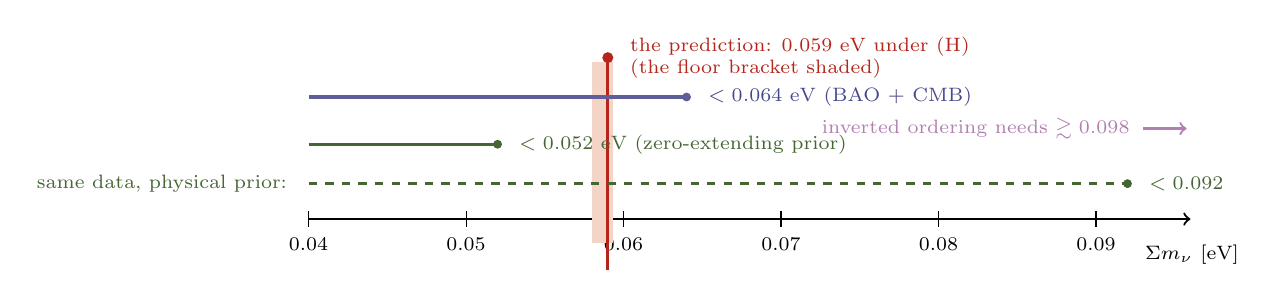
\begin{tikzpicture}[x=1cm, y=1cm]
% horizontal axis: Sum m_nu in eV, from 0.04 to 0.11
\draw[->, thick] (0,0) -- (11.2,0);
\foreach \x/\lab in {0/0.04, 2/0.05, 4/0.06, 6/0.07, 8/0.08, 10/0.09}{
  \draw (\x,0.1) -- (\x,-0.1);
  \node[font=\scriptsize, below] at (\x,-0.12) {\lab};
}
\node[font=\scriptsize, anchor=west] at (10.5,-0.45) {$\mnu$ [eV]};
% the framework's value 0.059 -> x = (0.059-0.04)*200 = 3.8; the floor bracket (0.0580, 0.0593) shaded
\fill[BrickRed!15] (3.6,-0.3) rectangle (3.86,2.0);
\draw[very thick, BrickRed] (3.8,-0.65) -- (3.8,2.05);
\fill[BrickRed] (3.8,2.05) circle (2pt);
\node[BrickRed, font=\scriptsize, anchor=west, align=left] at (3.96,2.05)
  {the prediction: $0.059$ eV under (H)\\ (the floor bracket shaded)};
% inverted floor at 0.098 -> x = 11.6 (off scale) ; draw arrow
\draw[Plum!80!black, thick, ->] (10.6,1.15) -- (11.15,1.15);
\node[Plum!80!black, font=\scriptsize, anchor=east] at (10.55,1.15)
  {inverted ordering needs $\gtrsim 0.098$};
% bound bars: shaded allowed region to the LEFT of each bound
\draw[MidnightBlue!70, very thick] (0,1.55) -- (4.8,1.55);
\fill[MidnightBlue!70] (4.8,1.55) circle (1.6pt);
\node[MidnightBlue!80, font=\scriptsize, anchor=west] at (4.95,1.55)
  {$< 0.064$ eV (BAO + CMB)};
\draw[OliveGreen!70!black, very thick] (0,0.95) -- (2.4,0.95);
\fill[OliveGreen!70!black] (2.4,0.95) circle (1.6pt);
\node[OliveGreen!70!black, font=\scriptsize, anchor=west] at (2.55,0.95)
  {$< 0.052$ eV (zero-extending prior)};
\draw[OliveGreen!70!black, very thick, dashed] (0,0.45) -- (10.4,0.45);
\fill[OliveGreen!70!black] (10.4,0.45) circle (1.6pt);
\node[OliveGreen!70!black, font=\scriptsize, anchor=west] at (10.55,0.45)
  {$< 0.092$};
\node[OliveGreen!70!black, font=\scriptsize, anchor=east] at (-0.15,0.45)
  {same data, physical prior:};
\end{tikzpicture}
\caption{The joint prediction, date-stamped (Observation \ref{prop:doublebet}, Remark \ref{rem:currency}). The framework predicts the sum at the normal-ordering floor, $0.059$ eV, under the hierarchical premise (H), with no free parameter: $w = -1$ is predicted. The shaded band is the floor's own bracket from the splittings, $0.0580$-$0.0593$ eV. Baryon-acoustic plus microwave data allow $\mnu < 0.064$ eV, slightly above the prediction. The tightest current combination reports $< 0.052$ eV, \emph{below} the floor, under a prior that extends to unphysical values; the same analysis with the physical floor imposed returns $< 0.092$ eV, and its authors read the excursion as a prior artefact rather than as physics, which is the reading this framework registers. Inverted ordering, requiring $\gtrsim 0.098$ eV, is the first to be excluded by the tightening, and is excluded here by rank in any case. All values are refreshed at submission; the prediction table of Section \ref{sec:bets} names what refutes what.}
\label{fig:bet}
\end{figure}

\begin{proposition}[Leptogenesis suppressed: the alignment, the reheating premise, and a new stance]\label{prop:leptogenesis}
The heavy neutrinos of Proposition \ref{prop:rankone} are the textbook mechanism of leptogenesis, and had that mechanism operated it would have generated the asymmetry in this tower alone, breaking the universality on which the dark-tower count and the arrow's accounting stand (Fact \ref{fact:ceiling}). The mechanism is suppressed in three steps, and the danger was double.
\begin{enumerate}
\item \emph{(The alignment result; proved.)} The decay asymmetry of the heavy state $N_{i}$ requires interference \cite{FukugitaYanagida1986, DavidsonNardiNir2008}, $\epsilon_{i} \propto \sum_{j \neq i}\mathrm{Im}\bigl[\bigl((Y_{D}^{\dagger}Y_{D})_{ij}\bigr)^{2}\bigr]\,f(M_{j}/M_{i})$, with $Y_{D}$ written in the heavy-mass eigenbasis. With $Y_{D} = y\J$ (Fact \ref{fact:democracy}) and $M_{R} = \alpha\mathbf{1} + \beta\J$ (Lemma \ref{lem:s3}), every heavy eigenbasis contains $u'$ (for $\beta \neq 0$, which the branch supplies; at $\beta = 0$ every basis is an eigenbasis and the conclusion holds a fortiori), and in any such basis the representation of $Y_{D}^{\dagger}Y_{D} = 3|y|^{2}\J$ has exactly one nonzero entry, on the diagonal at $u'$; every off-diagonal entry vanishes identically, so $\epsilon_{i} = 0$ for every $i$ at leading order, and the pair $N_{\perp}$ has no Dirac coupling at all. What this suppresses is the state $N_{u'}$; the pair is suppressed at leading order only because it does not couple.
\item \emph{(The degenerate pair, and the reheating premise.)} The graver threat was erasure, not production: the rank-one coupling washes exactly one lepton-flavour direction, the democratic one, with strength $K = m_{3}/m_{*} \approx 45$ for the equilibrium mass $m_{*} \in (1.06, 1.15)$ meV \cite{DavidsonNardiNir2008}, and a flavour-democratic descent asymmetry lies entirely in that direction; had the plasma ever reached $T \sim M_{3}$, the framework's own neutrinos would have erased the arrow's imprint. And the pair $N_{\perp}$, exactly degenerate at $\alpha$ at leading order, is the resonant configuration \cite{PilaftsisUnderwood2004}: after the breaking its couplings are $O(\delta)$ but the interference combination that controls its asymmetry, an off-diagonal entry of $Y_{D}^{\dagger}Y_{D}$ normalised by the two diagonal entries it connects, is $O(1)$ in $\delta$, so the pair's asymmetry is not switched off by the smallness of the breaking, and its value depends on the pair's split and widths, which this paper does not compute. What protects both is a premise, stated as such at the scale that does so:
\end{enumerate}
\begin{premise}[R: the descent reheats below the lower heavy scale]\label{prem:R}
$T_{\mathrm{desc}} \le \alpha = \min(\alpha, M_{3})$, with $\alpha$ on the branch of Remark \ref{rem:branch}. This is a reading of the dark-matter paper's own assumption (Fact \ref{fact:ceiling}: $T_{\mathrm{desc}}$ at the ceiling or below it) at "below"; under it no heavy state ever thermalised, the washout of $N_{u'}$ is Boltzmann-suppressed, the pair $N_{\perp}$ was never produced thermally, and the descent's $B - L$ is untouched. The natural justification, that the frozen phase's description dissolves above the rung scale, identifies $M_{3}$ with that scale, which is Hypothesis (U) and the valuation of Remark \ref{rem:valuation}, not a theorem; and (R) at $\alpha$ asks more of the descent than that, since $\alpha$ lies nearly two orders below $M_{3}$ on the branch taken. A derivation of $M$ and of $\alpha$ (successor problems (2) and (3)) would decide it.
\end{premise}
\begin{enumerate}
\setcounter{enumi}{2}
\item \emph{(The phases.)} Non-thermal decays of descent-populated heavy states inject asymmetry at order $\delta^{2}\sin\varphi$ from $N_{u'}$, and with an $O(1)$ prefactor times $\sin\varphi$ from the pair by (2), with $\delta$ the breaking of Lemma \ref{lem:breaking} and $\varphi$ a relative phase between the Dirac and Majorana matrices after it. Both matrices are built from one real geometric vacuum and one flavour-independent flag; the orientation is the only CP-violating mechanism the framework itself supplies (Fact \ref{fact:ceiling}, uniqueness not claimed there); that it is flavour-independent, one bit of the descent with no face index, as is the relaxing $\theta$-angle that Fact names as unexcluded, is this paper's reading of that object at observation level, and under it neither can generate a \emph{relative} phase between two family matrices; if the breaking is real in the vacuum's basis the relative phases vanish and the injection is zero to all orders in it. Under (R) a consistency consequence follows: the unification scale, on either of the Standard-Model paper's branches (Remark \ref{rem:valuation}), lies above $M_{3}$ at either end of Hypothesis (U), so the universe never revisited unification after the descent, and the meeting of the couplings, where there is one, is structural, not thermal history.
\end{enumerate}
The corollary is registered as the framework's fifth stance: the Dirac phase of lepton mixing is trivial, $\delta_{CP} \in \{0, \pi\}$. The current record leaves this allowed and, notably, allowed precisely in the ordering the framework predicts: the joint long-baseline analysis finds CP conservation allowed within the three-sigma interval for \emph{normal} ordering while excluding it at three sigma under \emph{inverted} ordering \cite{T2KNOvA2025}, so the stance's survival and the framework's ordering prediction are now the same experimental question. Should $\delta_{CP}$ prove nontrivial with normal ordering established, the real-breaking assumption fails, the double-beta values of Proposition \ref{prop:rankone}(3) revert to their hull, and subdominance would demand the injected asymmetry, $\delta^{2}\sin\varphi$ from $N_{u'}$ and $O(\sin\varphi)$ from the pair, below the asymmetry a successful leptogenesis needs, of order $10^{-7}$ in the standard treatments \cite{DavidsonNardiNir2008}, a tuning this framework would then have to record. (1) is proved at leading order; (2) is a premise; (3) is conditional on the real-breaking assumption.
\end{proposition}

\begin{proof}
\sloppy (1) Let $e_{1} = u'$, and $e_{2}, e_{3}$ any orthogonal basis of $u'^{\perp}$ (the $\alpha$-eigenspace is two-dimensional, so the choice is arbitrary and the conclusion cannot depend on it; the script uses $(1, -1, 0)$, $(1, 1, -2)$ and a second choice). Since $\J e_{2} = \J e_{3} = 0$ and $\J e_{1} = 3e_{1}$, the matrix $Y_{D}^{\dagger}Y_{D} = |y|^{2}\J^{\mathsf{T}}\J = 3|y|^{2}\J$ has, in this basis, one nonzero entry, at position $(1,1)$; in particular $(Y_{D}^{\dagger}Y_{D})_{ij} = 0$ whenever $i \neq j$ and $Y_{D}e_{2} = Y_{D}e_{3} = 0$. The script builds both bases exactly, transforms $Y_{D}^{\dagger}Y_{D}$ into them over the Gaussian rationals for complex $y$, and checks the six off-diagonal zeros and the vanishing of the $u'^{\perp}$ block of $Y_{D}$. (2) $K \in (43, 48)$ and the value $45$ from $m_{3}$ and $m_{*}$ bracketed (script). The resonant statement: with $Y_{D} = y(\J + \delta A)$ and $A$ complex, the script computes in the heavy eigenbasis, writing $T = Y_{D}^{\dagger}Y_{D}$ there, the ratio $|T_{23}|^{2}/(T_{22}T_{33})$ exactly at $\delta = 10^{-1}, 10^{-2}, 10^{-3}$ and finds it independent of $\delta$, while $|T_{12}|^{2}/T_{11}^{2}$ scales as $\delta^{2}$. The temperature statement is Premise (R). (3) With both matrices real in the vacuum's basis, every relative phase is zero and the injection's prefactor vanishes identically; the script parametrises a complex breaking by a unit Gaussian rational $e^{i\theta}$ and certifies that the interference term $\mathrm{Im}[((Y_{D}^{\dagger}Y_{D})_{1j})^{2}]$ between $N_{u'}$ and a member $j$ of the pair, in the heavy eigenbasis is zero at $\theta \in \{0, \pi\}$ and nonzero at $e^{i\theta} = (3 + 4i)/5$. The statement is exact in the real-breaking class and is flagged as conditional on it, which is what makes the corollary falsifiable. The consistency consequence is the scale comparison of Remark \ref{rem:valuation} at both ends.
\end{proof}

\subsection*{The prediction table: what decides what, and when}

The paper's stances, each with the measurement that refutes it. \emph{The sum.} A robust prior-independent $\mnu < 0.057$ eV within $w = -1$, across likelihoods and free of the lensing anomaly, refutes the joint prediction: the neutrino sector and the frozen-point cosmology cannot both survive. Live now, in successive baryon-acoustic and microwave releases \cite{DESI2025, HouWangZhaoZhang2026}. \emph{The ordering.} A confirmed inverted ordering refutes Proposition \ref{prop:rankone} outright; long-baseline and atmospheric data decide it, and cosmology already constrains inverted ordering most tightly. \emph{The lightest mass.} A determination of $m_{1}$ above about $1$ meV refutes Premise (H) as stated and moves the sum off the floor by more than the prediction's own margin; above about $4$ meV (certainly above $4.6$ meV, across the whole splitting bracket) the sum exceeds the $0.064$ eV bound already quoted, and a sum determined meaningfully above the floor, at $0.075$ eV say, refutes the prediction as decisively as one below it; neutrinoless double-beta decay at next-generation sensitivity refutes the rank-one structure itself. \emph{The phase.} A measured nontrivial $\delta_{CP}$ with normal ordering established refutes the real-breaking assumption of Proposition \ref{prop:leptogenesis}(3) and reopens the leptogenesis question it closed; the current joint analysis leaves it allowed under normal ordering and excluded under inverted \cite{T2KNOvA2025}. \emph{The orientation.} No completion of the orientation can exclude the identification, which is flag-covariant (Fact \ref{fact:ceiling}); there is no refutation condition here. The first of these may be the fastest-moving falsifier in the series, which is why this paper is written and dated now.

\subsection*{The levels of the results}

\emph{Proved in this paper, given the imported Facts:} the closed-form anomaly solution set and the anomaly invisibility of the total singlet (Proposition \ref{prop:empty}(2), (3)); the sixteenth refutation at its scope and the uniqueness of the neutral bilinear, an elementary statement (Proposition \ref{prop:seesaw}(1), (2)); the block inversion (Proposition \ref{prop:seesaw}(3)); the $S_{3}$ lemma (Lemma \ref{lem:s3}); the scalar seesaw on the democratic block and the rank-one light matrix (Proposition \ref{prop:rankone}(0)); the breaking relation (Lemma \ref{lem:breaking}); the alignment result at leading order (Proposition \ref{prop:leptogenesis}(1)).

\emph{Premises, named:} (M) the framework realises the Majorana term at $M \gg v$; (H) the second stage of the breaking is hierarchical, $m_{1}/m_{2} \lesssim 0.01$; (R) the descent reheats below $\alpha$; the real-breaking assumption of Proposition \ref{prop:leptogenesis}(3); the branch $\alpha \ll M_{3}$ of Remark \ref{rem:branch}; and, inherited, the Standard-Model paper's Hypothesis (S), the families paper's Conjecture 3.1 and its Gram-square reading (stated there for the condensate's source, extended here to the condensate-free $M_{R}$ as this paper's step, at structural level), the indifference instrument (a structural premise, applied here to $M_{R}$ at structural level), the dark-matter paper's Hypothesis (U) and Premise P4 and the gauge sector's CPT-evenness behind its flag covariance, and the dark-energy paper's condition on the frozen point.

\emph{Imported with provenance:} the derived content and the hypercharge per grade, the mass bracket and its charge, indifference, the faces and the democratic alignment, the exact join and the absence of a floor, the ceiling range and the flag covariance, and $w = -1$ (Facts \ref{fact:content}-\ref{fact:wminusone}); the unification scales of the Standard-Model paper, at its assembly level, and on its Pati-Salam route the chain's scales and the requirement on the neutrino sector, at record level (inline in Remarks \ref{rem:valuation} and \ref{rem:branch}); the oscillation splittings and angles, cosmological bounds, long-baseline and double-beta records \cite{PDG2024, NuFIT2024, DESI2025, HouWangZhaoZhang2026, T2KNOvA2025, KamLANDZen2023, LEGEND2021}, date-stamped and refreshed at submission.

\emph{Stances and readings, flagged:} the ordering (on the rank-one structure, itself on Fact \ref{fact:democracy} at its imported level); the sum (a kinematic lower bound for any $m_{1} \ge 0$; a prediction under (H)); the double-beta values (under (H) and the real-breaking assumption; a hull without it); the joint prediction (registered, at the level of its inputs); the $\delta_{CP}$ corollary (conditional on the real-breaking assumption, with its tuning cost quoted); the no-leading-order-mixing observation.

\subsection*{Successor problems}

Five. (1) \emph{The PMNS numbers:} all three angles are second-order effects here, depending on the same breaking that the CKM numbers depend on, and therefore on the families paper's second-order programme and its registered open problem \cite[Prop.~4.3(4), Obs.~7.1]{ButlerT13}; the large angles are the most demanding requirement on that breaking. (2) \emph{The two light masses and $\alpha$ at second order:} compute how far the two stages of the breaking lift $m_{2}$ and $m_{1}$, and what fixes $\alpha$, which would decide Premise (H), test the relation of Remark \ref{rem:branch}, and convert the double-beta values into a single prediction; on the Standard-Model paper's Pati-Salam route the question becomes whether the family structure that fits the charged fermions there gives this branch. (3) \emph{Deriving $M$:} identify the framework's object that realises the neutral bilinear (Fact \ref{fact:bracket} says nothing about it: the bracket is computed there only on slot states) and obtain its scale from its own dynamics rather than from the observed masses under Hypothesis (U), discharging Premise (M), deciding Premise (R), and turning the agreement with the dark-matter paper's rung scale from a construction into a check. (4) \emph{The degenerate pair and the non-thermal injection:} compute the split and widths of $N_{\perp}$ after the breaking, and bound the injected asymmetry ($\delta^{2}\sin\varphi$ from $N_{u'}$, $O(\sin\varphi)$ from the pair) from the descent's own dynamics rather than from the real-breaking assumption, which would convert the fifth stance from conditional to derived. (5) \emph{Dataset currency:} this paper's numbers are date-stamped by construction; the prediction table above is the object to refresh, and the capstone maintains the series-wide version.

\section{Position in the series}\label{sec:position}

This paper is T15 of the series. \emph{It relies on six predecessors:} the root paper T1 \cite{ButlerT1} for the transport principle and the series' method; the dark-energy paper T10 \cite{ButlerT10} for the registered $w = -1$ with its condition (Fact \ref{fact:wminusone}); the mass paper T11 \cite{ButlerT11} for the exact join, with its massless locus in place of a floor, and the bracket's dimensions (Fact \ref{fact:join}); the Standard-Model paper T12 \cite{ButlerT12} for the derived content, the hypercharge per grade, the mass bracket's quantum numbers, the unification scale on its conditional branch and the unconditional pairwise meetings (\cite[Prop.~6.2]{ButlerT12}, at that paper's assembly level, cited inline in Remark \ref{rem:valuation}), the Pati-Salam chain's scales and the requirement it places on the neutrino sector (\cite[Props.~10.10, 11.2]{ButlerT12}, at record level, inline in the same remark), and Hypothesis (S), on which this paper's doublet content depends and which it records as open (Facts \ref{fact:content}, \ref{fact:bracket}); the families paper T13 \cite{ButlerT13} for the indifference instrument, the faces, the democratic alignment and its registered open problem (Fact \ref{fact:democracy}, Observation 7.1 there); and the dark-matter paper T14 \cite{ButlerT14} for the ceiling range under Hypothesis (U), the arrow as a declared stance with Premise P4, the flag covariance, and the reheating assumption (Fact \ref{fact:ceiling}).

\emph{Papers that rely on this one:} the dark-matter paper T14 \cite{ButlerT14} cites the sixteenth refutation (Proposition \ref{prop:seesaw}(1), whose scope is the cosmological term of the deformed bracket, not a floor) and the flag covariance of the $\nu_{R}$ identification, $\nu_{R}$ being the hypercharge-zero singlet at grade zero of T12's listing (Proposition \ref{prop:empty}); its seeding appendix's reheating is read here at the lower heavy scale (Premise (R)), about two to five orders below the top of the range across which that appendix quotes its numbers, so the numbers quoted at the top of that range do not apply on this paper's branch; the mass paper T11 \cite{ButlerT11} refers the massless locus of its join to this paper; the families paper T13 \cite{ButlerT13} refers to this paper the neutrino exemption from its Koide relation, whose mechanism (seesaw-composed masses) holds under Premise (M); the capstone T17 \cite{ButlerT17} tabulates this paper's claims at their tiers, carries the sixteenth refutation in its refutation table at the scope of Proposition \ref{prop:seesaw}(1), numbers the framework's stances (the joint prediction fourth, the phase fifth), and maintains the series-wide table of falsifiable claims of which Section \ref{sec:bets} is the neutrino sector's entry; what it takes from this paper is the refutation at that scope (the cosmological term, not a floor), the seesaw as premised under (M) rather than derived, the empty twistor at grade zero, the branch of Remark \ref{rem:branch}, and Premises (M), (H), (R) with the results that depend on each.

\section{Machine verification}\label{sec:verification}

Every computational identity asserted in this paper at its own proof level, with the exceptions listed at the end, has been verified in exact arithmetic by the script \texttt{verify\_T15.py} \cite{ButlerVerifyT15}, which imports the series' shared library \texttt{GA.py}: exact rationals, Gaussian rationals with exact linear algebra, and certified rational interval arithmetic (integer square roots with proved brackets) for the measured splittings, the mixing angles, the top and bottom masses, the equilibrium mass, and the physical constants. No floating point is used anywhere. Every observational input behind a quoted number enters as a bracket, printed in the text where the input is used, so a refresh changes the inputs and not the logic; the light charged-fermion masses ($e, \mu, \tau, u, c$) enter at their central values, used for one-significant-figure ratios except $m_{\mu}/m_{\tau}$, whose three figures calibrate $\delta_{c}$ and which the script ties to those masses; and $M_{U}$ enters at the two values the text names, $2 \times 10^{16}$ GeV (the ratios) and $7 \times 10^{14}$ GeV (the factor $1.16$-$1.19$); the Pati-Salam chain's values enter as the brackets $v_{R} \in (4.1, 4.2) \times 10^{10}$ GeV and $M_{I} \in (1.9, 2.0) \times 10^{10}$ GeV, with $M_{U} = 3.36 \times 10^{16}$ GeV and $m_{t}(M_{I}) = 92$ GeV, as the Standard-Model paper records them.

\emph{Part A: the empty twistor.} The graded dimensions $1, 3, 3, 1$ of $\Lambda^{\bullet}\C^{3}$ with its two singlets; the hypercharge per grade under the weight rule, with $Y = 0$ at grade zero and $Y = -1$ at grade three; the four anomaly sums on the derived spectrum; the closed-form solution set $(a, 2a - f, f - 4a, -3a, 6a - f, f)$ satisfying all four sums for several $(a, f)$; the reduction of the cubic sum to $18a(8a^{2} + bc - 6af + f^{2})$ under the linear conditions; the linear decomposition of the closed form into $6Y$ and $(B - L) - 2Y$, which is the two-dimensional span; the family $Y + t(B - L)$ at $t = 1, -1, 2, \tfrac57$ with $Y_{N} = t$, the vanishing of all four sums on $B - L$, and the two mixed cubic coefficients zero; the collapse to the unique solution at $Y_{N} = 0$; the four sums recomputed over an explicit five-state spectrum with the singlet deleted, equal to the six-state sums at $Y_{N} = 0$ and unequal at $Y_{N} \neq 0$; the ray $B - L$ anomaly-free with $Y_{N}/Y_{Q} = 3$ and outside the family; and the $\mathbb{Z}_{6}$ condition as a function over the whole derived content, with an off-lattice hypercharge failing it.

\emph{Part B: the seesaw.} The $\Lambda$-term neutrino's extent $l/\LH = 2^{1/4}$ exactly for $p = m$, and $l \in (1.3, 1.5) \times 10^{20}$ m for $p = 100$ GeV from $\Lambda \in (1.0, 1.2) \times 10^{-52}$ m$^{-2}$; the Casimir $C \in (1.6, 2.0) \times 10^{63}$; the neutral-bilinear census over all twenty-one pairs; the block elimination identity assembled on rational instances and the scalar small eigenvalue certified within $m_{D}^{4}/M_{R}^{3}$ of $-m_{D}^{2}/M_{R}$; the $S_{3}$ lemma (characterisation on positive and negative instances over all six permutations, the spectrum, the determinant with both singular loci, the inverse against the adjugate, the projector form); the block decomposition of Proposition \ref{prop:rankone}(0), the identity $\J M_{R}^{-1}\J = 3M_{3}^{-1}\J$ and the light matrix on several $(\alpha, \beta, d)$; rank preservation for a rank-one $\mD$ across non-$S_{3}$-invariant invertible $M_{R}$; the shared heavy eigenvector $u'$; the exact identity of Lemma \ref{lem:breaking} on rational instances; the light matrix diagonalised exactly at the $S_{3} \to S_{2}$ direction, with $m_{2}/m_{3} \in (0.168, 0.172)$ at $\delta = 0.286$, $M_{3}/\alpha = 66$ (an instance chosen to land on the measured ratio, not a test of it), the charged-sector calibration $\delta_{c} = 0.286$ from $m_{\mu}/m_{\tau}$ by exact singular values (the target tied to the script's own lepton masses), the leading-order $\delta' = 0.024$ against the diagonalised $1/66$, the non-monotonicity of the exact ratio in $M_{3}/\alpha$ (its value at $176$ exceeding those at $66$ and at $500$, and the second root's existence between them), the small-$\delta$ convergence to the $\lambda_{A} = \tfrac49$ formula, and the compression eigenvalues $\lambda_{A} = \tfrac49$, $\lambda'_{A} = 0$; the inverted ratio $m_{1}/m_{2} > 0.98$; the floor inside $(0.0580, 0.0593)$ eV, the sum at $m_{1} = 0.1, 1, 3, 10$ meV, the value at $m_{1} = 8.7$ meV ($m_{1}$ of order $m_{2}$) above $0.07$ eV, the crossing of the $0.064$ eV bound between $3.5$ and $4.6$ meV, the inverted floor inside $(0.097, 0.102)$ eV, and $m_{2}/m_{3} \in (0.16, 0.18)$; the $0.052$ eV bound below the floor; the two double-beta values from the angle and splitting brackets, their shift below $0.1$ meV at $m_{1} = 0.1$ meV, and the four sign patterns at $m_{1} = 1$ meV spanning $0.6$-$4.6$ meV; the valuation of $M_{3}$ at both ends of Hypothesis (U) from the quark-mass brackets, $(m_{t}/m_{b})^{2} \in (1.6, 1.8) \times 10^{3}$, the two unification ratios at $2 \times 10^{16}$ GeV and the factor $1.16$-$1.19$ at $7 \times 10^{14}$ GeV; the charged-sector ratios $m_{\mu}/m_{\tau}$, $m_{e}/m_{\mu}$, $m_{u}/m_{c}$ from the record; the mixing requirement $|U_{\tau 3}|^{2} \in (0.39, 0.55)$; and $\alpha$ at both ends of (U) on the branch; on the Pati-Salam branch, $\sqrt{m_{3}v_{R}}$ inside $(1.42, 1.46)$ GeV, which is the requirement's coefficient $1.44$, the coupling a top-like $m_{D}$ would need inside $(3900, 4200)$, and the ordering $\alpha_{\mathrm{bottom}} < M_{I} < \alpha_{\mathrm{top}}$ with $M_{U}$ above $M_{3}$ at both ends.

\emph{Part C: leptogenesis.} The alignment result in two exact eigenbases of $u'^{\perp}$ over the Gaussian rationals for complex $y$; the resonant ratio for the degenerate pair independent of $\delta$ while the $N_{u'}$ ratio scales as $\delta^{2}$; the washout strength $K \in (43, 48)$ from bracketed $m_{3}$ and $m_{*}$; and the interference term with a complex breaking phase, zero at $0$ and $\pi$ and nonzero off them.

What the script does not check, imported or premised at the cited levels: the measurements themselves \cite{PDG2024, NuFIT2024, DESI2025, HouWangZhaoZhang2026, T2KNOvA2025, KamLANDZen2023, LEGEND2021}, including the $0.064$, $0.052$, $0.057$, $0.092$ and $0.111$ eV bounds and the double-beta limit and projection, which are quoted; the standard Boltzmann treatment behind $m_{*}$ and the order-$10^{-7}$ asymmetry a successful leptogenesis needs; the dimensional analysis of Fact \ref{fact:join}, which is read from T11's conventions; the application of the indifference instrument to $M_{R}$ and the extension of the Gram-square reading to it, at the level Fact \ref{fact:democracy} holds them; the extension of face-valuedness to the $LN$ bracket; the two remainders in Lemma \ref{lem:breaking}, $O(\delta)$ and $O(\delta^{2}M_{3}/\alpha)$, which are argued in the proof and instanced, not certified in general; the tilt estimates and the degree conversion of Observation \ref{obs:mixing}; the flavour-independence reading of Proposition \ref{prop:leptogenesis}(3); and Premises (M), (H) and (R) and the branch of Remark \ref{rem:branch}, which are premises.

\begin{thebibliography}{99}

\bibitem{ButlerT1}
L.~Butler,
\emph{The Transport Principle: Total Division in Clifford Algebras via Minimal Completion},
Transport Papers T1 (2026).

\bibitem{ButlerT10}
L.~Butler,
\emph{Dark Energy and the Action of Gravity: MacDowell-Mansouri, the Frozen Point, and One Way to Grip},
Transport Papers T10 (2026).

\bibitem{ButlerT11}
L.~Butler,
\emph{The Origin of Mass: The Weight Dictionary and the Exact Join},
Transport Papers T11 (2026).

\bibitem{ButlerT12}
L.~Butler,
\emph{The Standard Model from the Minimal Massive Composite},
Transport Papers T12 (2026).

\bibitem{ButlerT13}
L.~Butler,
\emph{Quark and Lepton Families: Condensation, Democracy, and the Koide Relation},
Transport Papers T13 (2026).

\bibitem{ButlerT14}
L.~Butler,
\emph{Dark Matter and the Arrow of Time: The Five Dark Towers},
Transport Papers T14 (2026).

\bibitem{ButlerT17}
L.~Butler,
\emph{The Transport Programme: Method, Status, and the Falsifiable Ledger},
Transport Papers T17 (2026).

\bibitem{Minkowski1977}
P.~Minkowski,
\emph{$\mu \to e\gamma$ at a rate of one out of $10^{9}$ muon decays?},
Phys. Lett. B \textbf{67} (1977), 421--428.

\bibitem{GRS1979}
M.~Gell-Mann, P.~Ramond, and R.~Slansky,
\emph{Complex spinors and unified theories},
in \emph{Supergravity}, North-Holland (1979), 315--321.

\bibitem{Yanagida1980}
T.~Yanagida,
\emph{Horizontal symmetry and masses of neutrinos},
Prog. Theor. Phys. \textbf{64} (1980), 1103--1105.

\bibitem{MohapatraSenjanovic1980}
R.~N. Mohapatra and G.~Senjanovi\'c,
\emph{Neutrino mass and spontaneous parity nonconservation},
Phys. Rev. Lett. \textbf{44} (1980), 912--915.

\bibitem{HHW1978}
H.~Harari, H.~Haut, and J.~Weyers,
\emph{Quark masses and Cabibbo angles},
Phys. Lett. B \textbf{78} (1978), 459.

\bibitem{FukugitaYanagida1986}
M.~Fukugita and T.~Yanagida,
\emph{Baryogenesis without grand unification},
Phys. Lett. B \textbf{174} (1986), 45--47.

\bibitem{DavidsonNardiNir2008}
S.~Davidson, E.~Nardi, and Y.~Nir,
\emph{Leptogenesis},
Phys. Rep. \textbf{466} (2008), 105--177.

\bibitem{PilaftsisUnderwood2004}
A.~Pilaftsis and T.~E.~J.~Underwood,
\emph{Resonant leptogenesis},
Nucl. Phys. B \textbf{692} (2004), 303--345.

\bibitem{PDG2024}
S.~Navas et al. (Particle Data Group),
\emph{Review of particle physics},
Phys. Rev. D \textbf{110} (2024), 030001. % refresh at submission.

\bibitem{NuFIT2024}
I.~Esteban, M.~C.~Gonzalez-Garcia, M.~Maltoni, I.~Martinez-Soler, J.~P.~Pinheiro, and T.~Schwetz,
\emph{NuFit-6.0: updated global analysis of three-flavor neutrino oscillations},
J. High Energy Phys. \textbf{12} (2024), 216, arXiv:2410.05380. % refresh at submission: the splitting and angle brackets.

\bibitem{DESI2025}
M.~Abdul Karim et al. (DESI Collaboration),
\emph{DESI DR2 results II: measurements of baryon acoustic oscillations and cosmological constraints},
preprint arXiv:2503.14738 (2025). % refresh at submission; the 0.064 eV bound and the live dataset of the joint bet.

\bibitem{HouWangZhaoZhang2026}
H.~Hou, S.~Wang, Z.-C.~Zhao, and X.~Zhang,
\emph{Constraints on the sum of neutrino masses from ACT DR6 and DESI DR2 considering isocurvature initial conditions},
preprint arXiv:2606.17994 (2026). % refresh at submission: 0.052 eV (LCDM, adiabatic, zero-extending prior), 0.057 eV (with isocurvature), 0.092 eV (physical floor), 0.111 eV (w0wa, adiabatic).

\bibitem{T2KNOvA2025}
K.~Abe et al. (T2K Collaboration) and M.~A. Acero et al. (NOvA Collaboration),
\emph{Joint neutrino oscillation analysis from the T2K and NOvA experiments},
Nature (2025). % refresh at submission with volume, pages and DOI: CP conservation allowed under normal ordering, excluded at three sigma under inverted.

\bibitem{KamLANDZen2023}
S.~Abe et al. (KamLAND-Zen Collaboration),
\emph{Search for the Majorana nature of neutrinos in the inverted mass ordering region with KamLAND-Zen},
Phys. Rev. Lett. \textbf{130} (2023), 051801. % the current limit, m_bb < 28-122 meV.

\bibitem{LEGEND2021}
N.~Abgrall et al. (LEGEND Collaboration),
\emph{The Large Enriched Germanium Experiment for Neutrinoless $\beta\beta$ Decay: LEGEND-1000 preconceptual design report},
preprint arXiv:2107.11462 (2021). % the next-generation projection, m_bb reach near 10 meV.

\bibitem{ButlerVerifyT15}
L.~Butler,
\emph{verify\_T15.py: machine verification for ``Neutrino Masses''},
Python script, deposited with this paper alongside the shared library GA.py (2026).

\end{thebibliography}

\end{document}
